\chapter{Synthetic Nervous System Simulation}\label{ch:sns}
\graphicspath{{../Figures/60-sns/}{../Figures/60-sns/AnimatLab_reference/}}

% [ZCODE 2026-10-15 Phase-A restructure: sections moved verbatim from the former monograph chapters; provenance in Notes/revision_campaign_20261015/migration_map.md]

\section{Preliminary Neuromechanical Simulation Workflows}\label{sec:preliminary_sim_methods}

Preliminary simulation workflows were assembled to support future integration of the BPA mechanics and synthetic nervous system (SNS). The figures in this section document the biomechanical representations, controller organization, and software implementation. Their purpose is to identify what was constructed; quantitative validation remains separate.

\subsection{AnimatLab Body and Controller Organization}

The walker representation and controller hierarchy are shown in Figures~\ref{fig:animatlab_model_architecture} and~\ref{fig:animatlab_working_gui}. The hierarchy separates rhythm generation, hip control, and knee--ankle pattern formation within left- and right-side neural subsystems. The current AnimatLab working model was instrumented for a new \qty{10}{\second} phase-1 run recording joint, neural, contact-sensory, and body-motion channels. This run was used to inspect recorded signals and simulation behavior, without treating it as evidence of stable walking or effective ground-contact gating. It is distinct from the earlier walker study described in Section~\ref{sec:prior_walker}. Preliminary joint-motion results are reported in Section~\ref{sec:preliminary_sim_results}.

Since that run, the working model has been reorganized into a complete bilateral network. The right-side rhythm-generator, hip, and knee--ankle subsystems were mirrored from the left, inhibitory commissural pathways were added between the two rhythm generators, and each leg gained four biarticular muscle pathways (gastrocnemius, biceps femoris short head, semimembranosus, and rectus femoris) with human maximum isometric forces from the Gait2392 data set. The reorganized project opens in the AnimatLab environment without errors and exports a standalone simulation that runs headless. Its rhythm-generator half-centers hold a static latch under the tonic drive levels tested so far rather than oscillating, so conductance tuning toward robust oscillation is the active step; no locomotor claim is made for the reorganized model beyond its verified assembly.

Figure~\ref{fig:animatlab_controller_motifs} illustrates the rhythm-generator, pattern-formation, and sensorimotor organization at the neuron and synapse level. These reference schematics complement the subsystem view by making the antagonist pathways and sensory connections visible.

\begin{figure}[p]
\centering
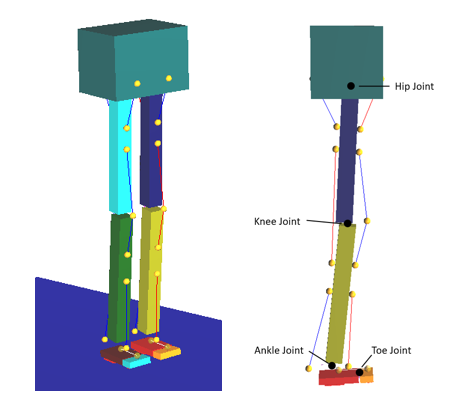
\includegraphics[width=0.64\textwidth,height=0.30\textheight,keepaspectratio]{OurWalker.png}
\par\medskip
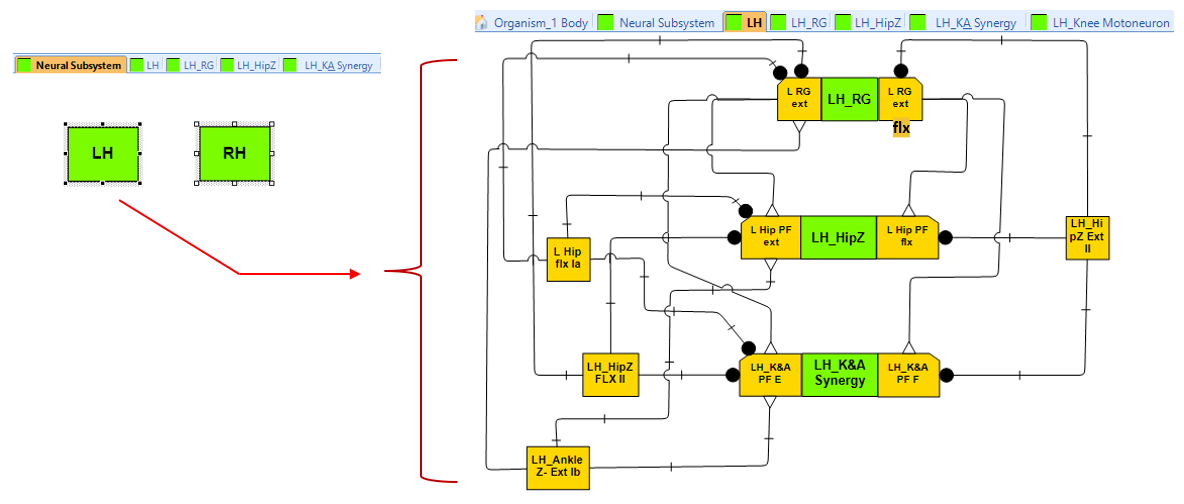
\includegraphics[width=\textwidth,height=0.31\textheight,keepaspectratio]{2layerImprove.png}
\caption[AnimatLab walker and controller hierarchy]{AnimatLab model and architecture illustrations. Top: the segmented walker and labeled hip, knee, ankle, and toe joints. Bottom: the left/right subsystem organization and an expanded view of the left-side rhythm-generator, hip, and knee--ankle modules. These architectural views describe model organization and are not snapshots of the phase-1 trajectory.}
\label{fig:animatlab_model_architecture}
\end{figure}

\begin{figure}[p]
\centering
\begin{minipage}[t]{0.47\textwidth}\centering
\textbf{(A) Rhythm generator}\par\smallskip
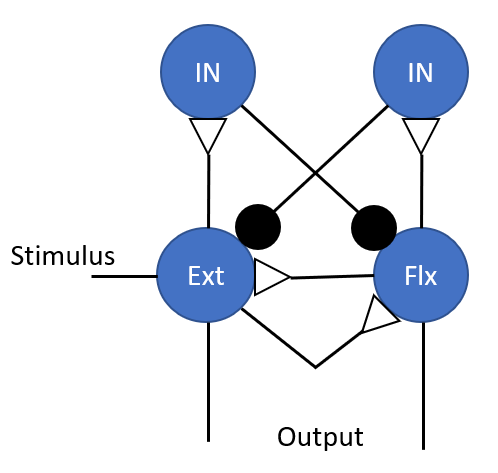
\includegraphics[width=\linewidth,height=0.20\textheight,keepaspectratio]{RGnetwork.PNG}
\end{minipage}\hfill
\begin{minipage}[t]{0.47\textwidth}\centering
\textbf{(B) Pattern formation}\par\smallskip
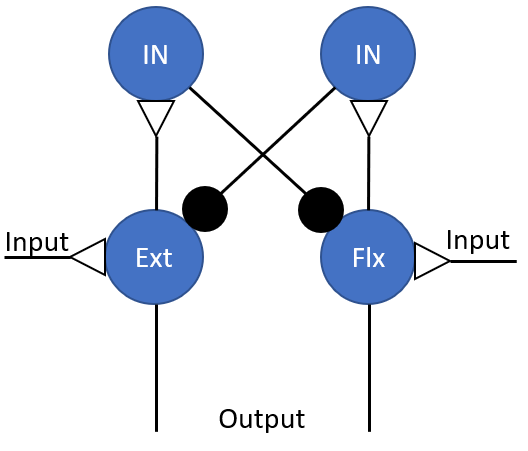
\includegraphics[width=\linewidth,height=0.20\textheight,keepaspectratio]{PFnetwork.PNG}
\end{minipage}
\par\medskip
\textbf{(C) Sensorimotor organization}\par\smallskip
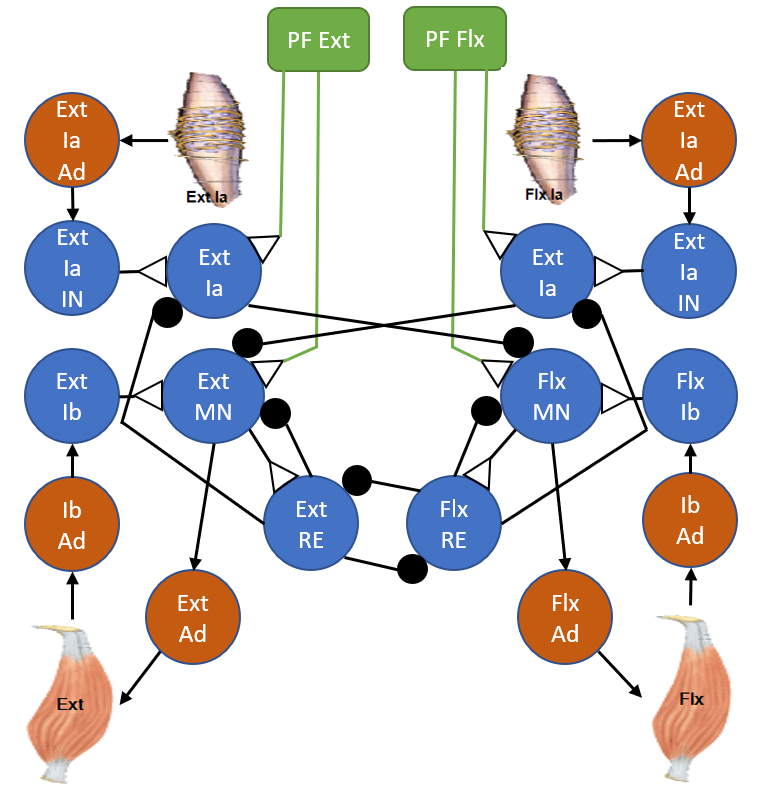
\includegraphics[width=0.76\textwidth,height=0.39\textheight,keepaspectratio]{sensoryMotor_Network.PNG}
\caption[AnimatLab controller reference schematics]{Reference schematics of \textbf{(A)} rhythm generation, \textbf{(B)} pattern formation, and \textbf{(C)} sensorimotor organization. Ext and Flx identify antagonist extensor and flexor pathways; IN denotes interneurons, MN motor neurons, and Ia and Ib muscle afferent pathways. Open triangles and filled circles distinguish excitatory and inhibitory synaptic connections. These schematics illustrate controller architecture and are not readouts from the phase-1 run.}
\label{fig:animatlab_controller_motifs}
\end{figure}

\begin{figure}[p]
\centering
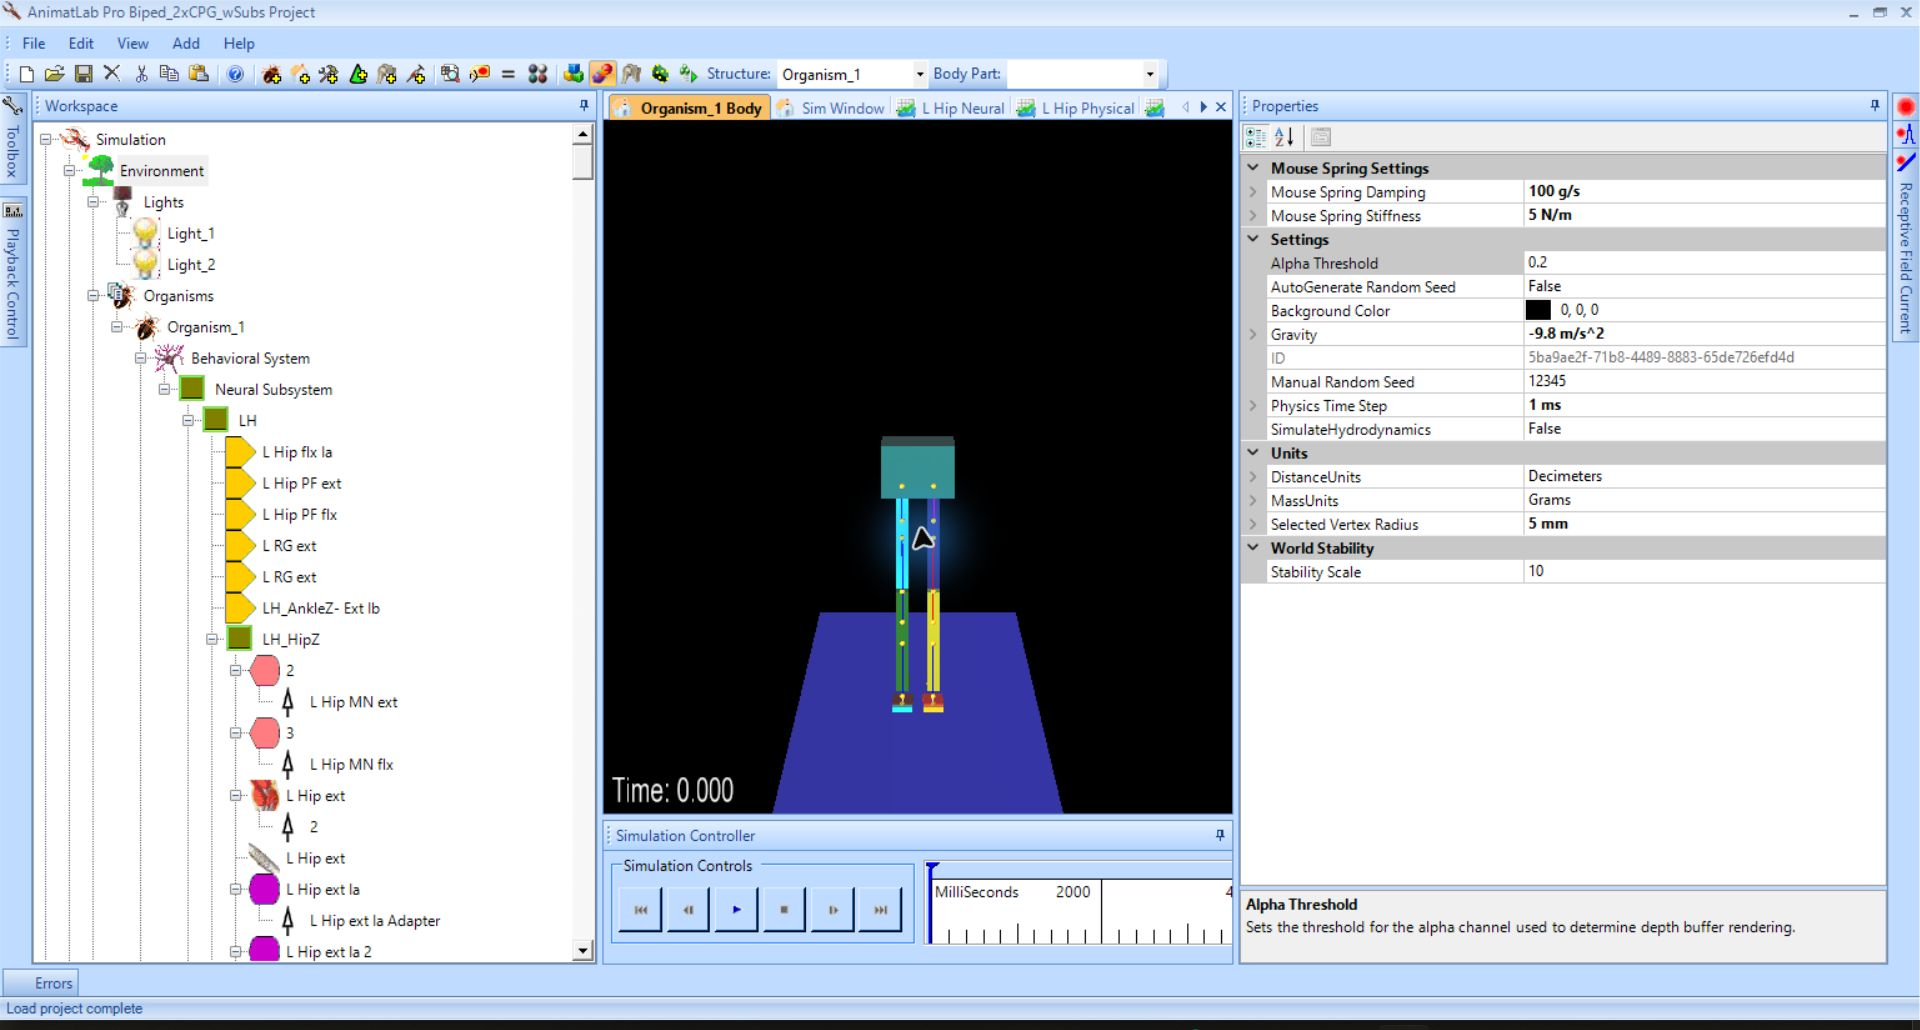
\includegraphics[width=\textwidth,height=0.31\textheight,keepaspectratio]{animatlab_body_gui.png}
\par\medskip
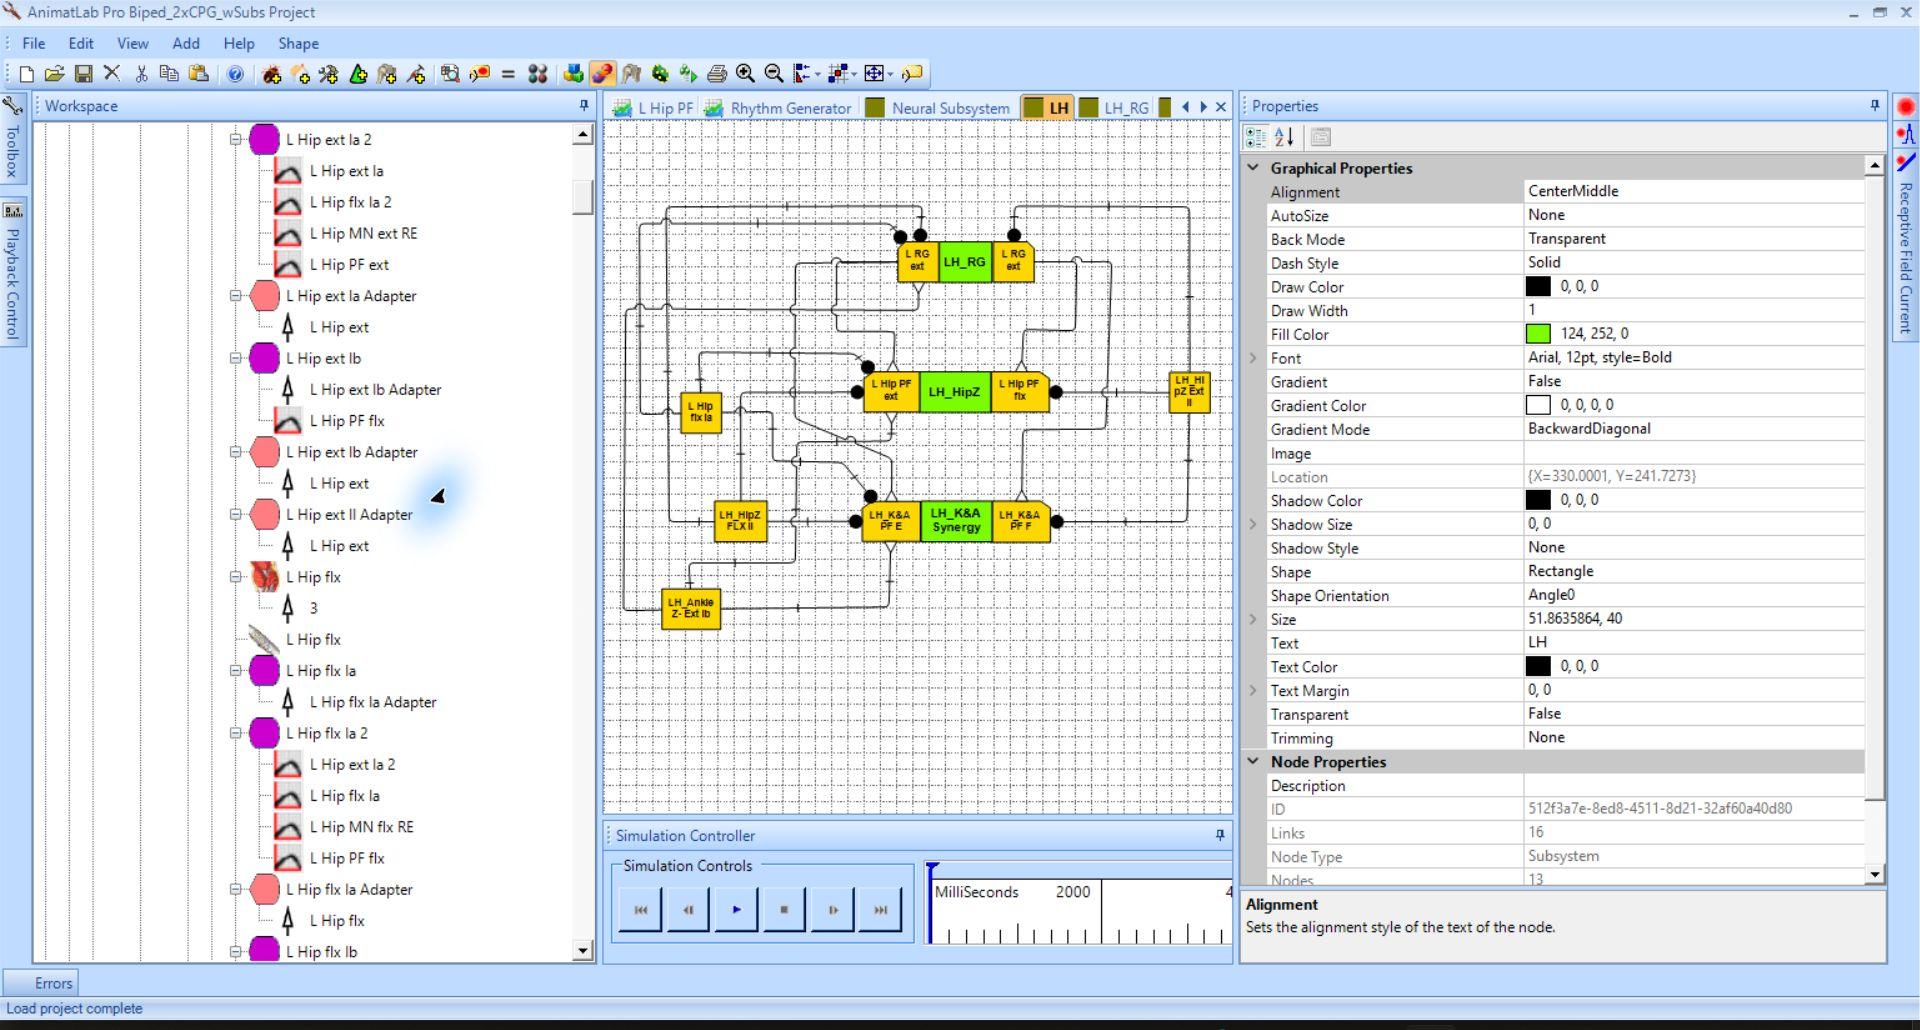
\includegraphics[width=\textwidth,height=0.31\textheight,keepaspectratio]{animatlab_network_gui.png}
\caption[AnimatLab working-project interface]{The saved AnimatLab working project opened in the application: the biomechanical body at initialization (top) and the expanded left-side controller subsystem (bottom). The workspace tree and property inspector expose the relationship between the body, sensory pathways, and neural modules. These interface captures were acquired without running a new simulation.}
\label{fig:animatlab_working_gui}
\end{figure}

\subsection{MuJoCo Conversion and Synthetic BPA Knee}

A reproducible OpenSim-to-MuJoCo conversion workflow was assembled using scripted model repair, MyoConverter, and a documented software environment. Separately, a custom quasi-static BPA model was ported from MATLAB to Python and coupled to MuJoCo tendon kinematics to compute actuator forces and their joint contributions. A minimal SNS with reciprocal inhibition drove a synthetic knee with antagonistic flexor and extensor BPAs. Figure~\ref{fig:mujoco_model_views} distinguishes the converted robot from this separate knee demonstration. The demonstration establishes a controller--actuator--joint interface; it does not establish SNS control of the converted Gait2392 robot or validation of correction-factor-based MuJoCo torque predictions.

At the time of writing the conversion stage is complete and verified: the converted model carries all 92 muscle-tendon actuators with attachment geometry audited against the OpenSim source, and the joint sign conventions of the robot's modified paths were audited dynamically (from simulation torques rather than static model tables, because coupled path points move). The BPA port reproduces the MATLAB force calculation, including the correction-factor force balance. An SNS-Toolbox network couples to MuJoCo at a \qty{0.1}{\milli\second} neural step, with muscle force feedback entering as Ib afferent input. On this coupling, a 406-neuron two-layer spinal network has been assembled for the converted model --- per-leg rhythm-generator half-centers, four phase-shifted pattern-formation groups per leg, motoneuron pools for all actuators, and Ia, Ib, and II afferent populations --- and its rhythm generator has been verified in isolation to oscillate at an approximately \qty{0.9}{\second} cycle with the two legs in antiphase under tonic drive. Full-body closed-loop co-simulation is not yet running: leg-joint states develop non-finite values during longer simulations, with the foot-contact meshes the primary suspect under investigation.

\begin{figure}[p]
\centering
\begin{minipage}[t]{0.48\textwidth}\centering
\textbf{(A) Converted robot}\par\smallskip
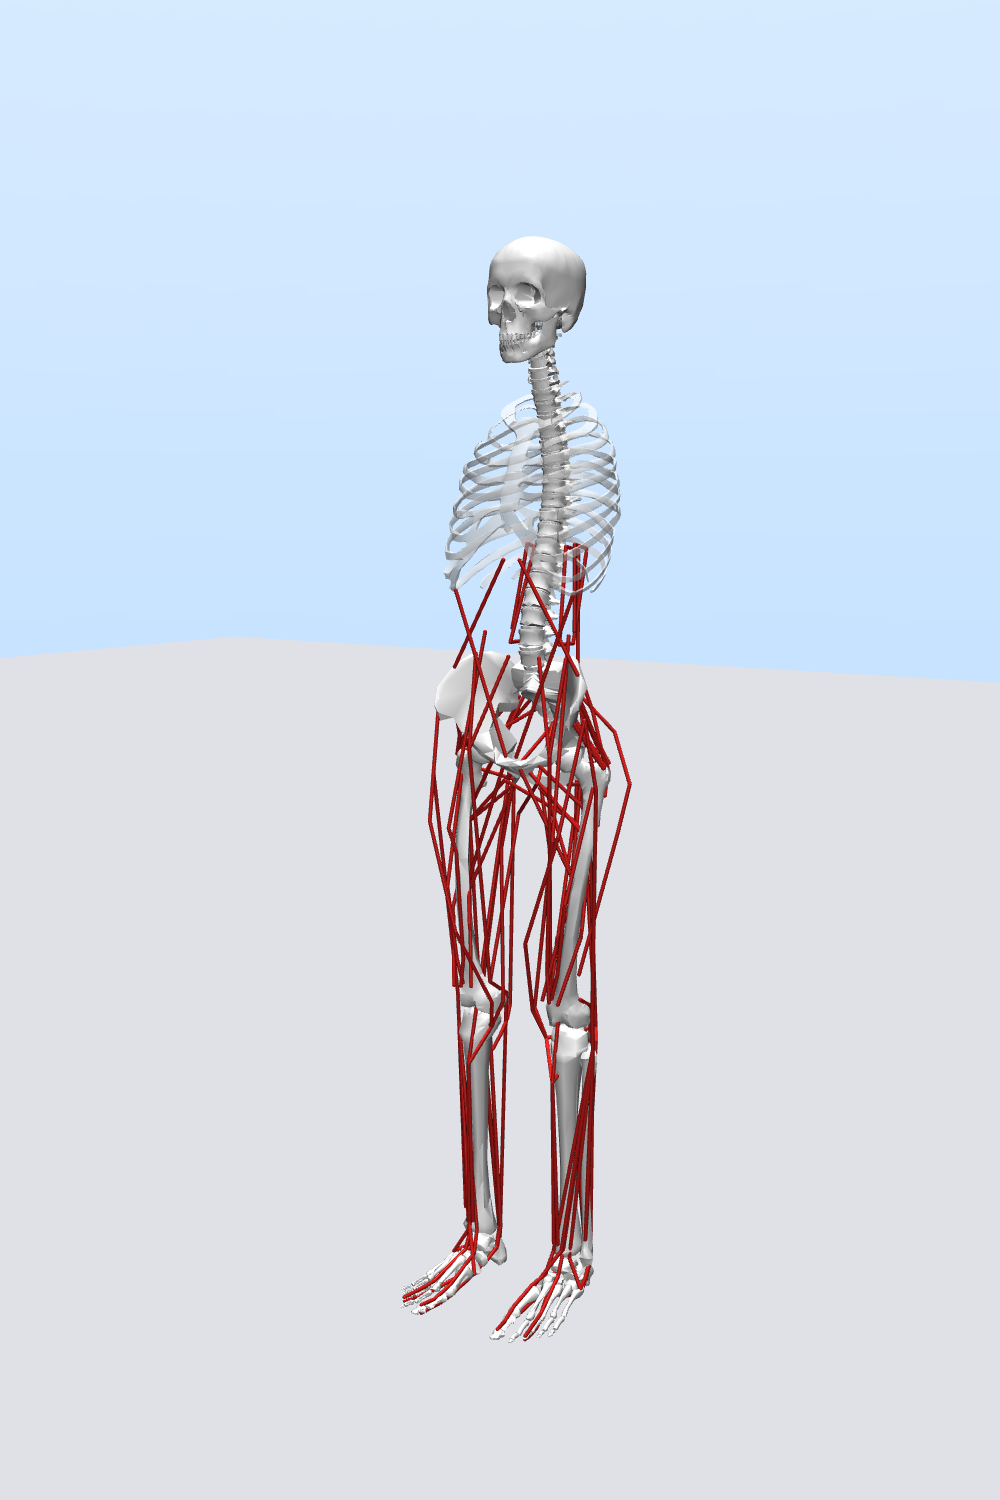
\includegraphics[width=\linewidth,height=0.53\textheight,keepaspectratio]{mujoco_converted_robot.png}
\end{minipage}\hfill
\begin{minipage}[t]{0.48\textwidth}\centering
\textbf{(B) Synthetic BPA knee}\par\smallskip
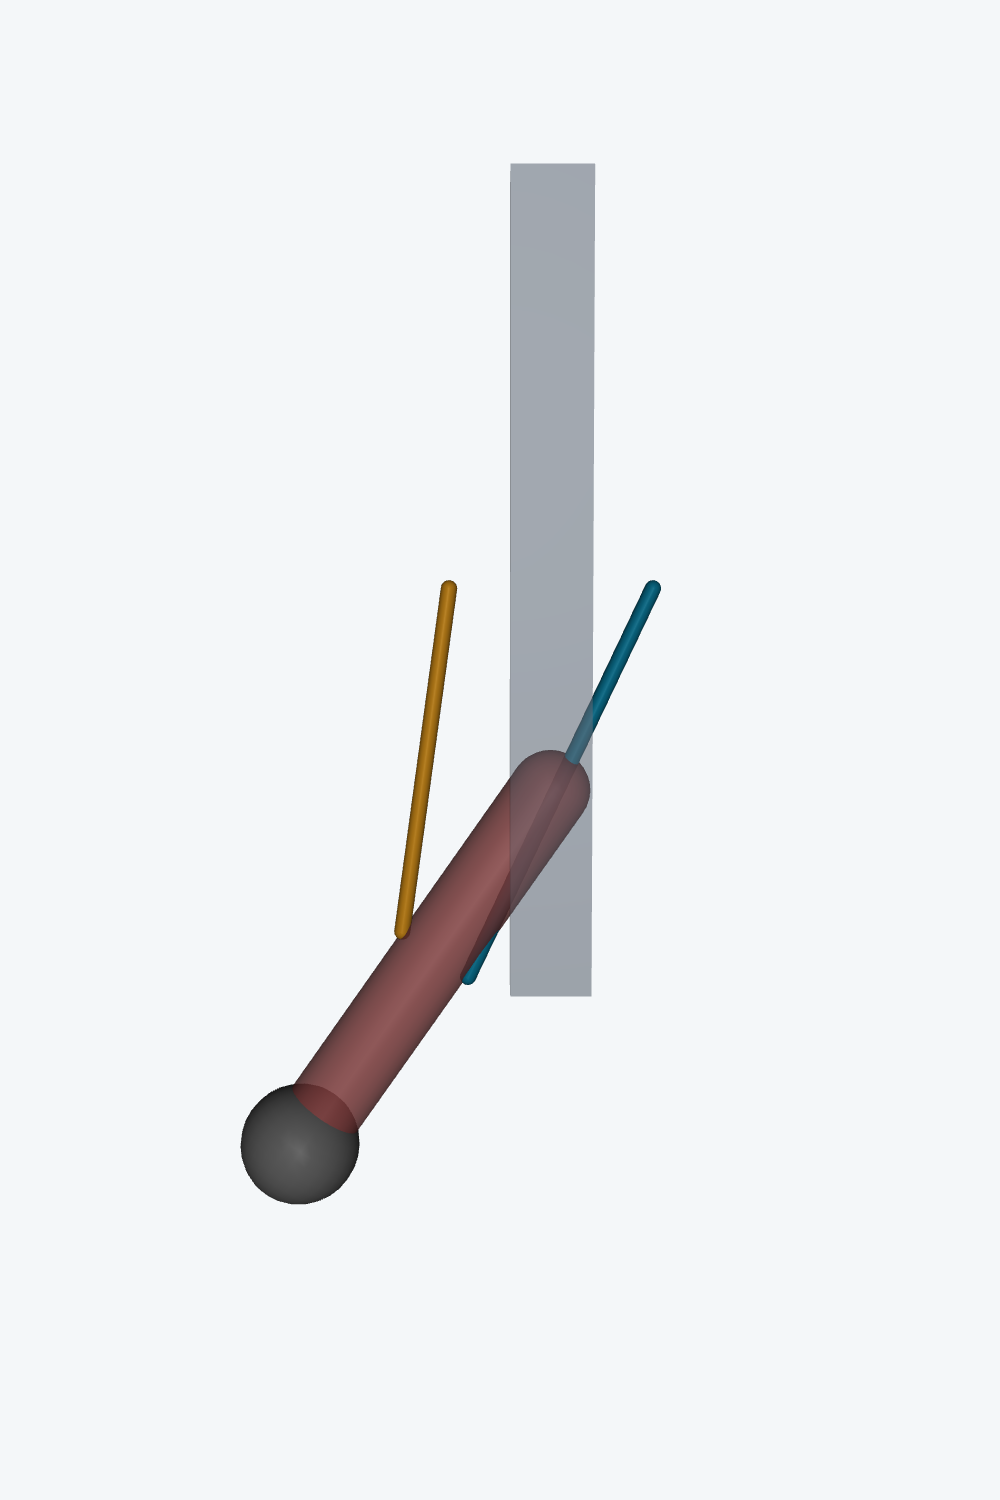
\includegraphics[width=\linewidth,height=0.53\textheight,keepaspectratio]{mujoco_synthetic_knee.png}
\end{minipage}
\caption[MuJoCo model representations]{Native MuJoCo renders of \textbf{(A)} the converted Gait2392 robot at its saved reference pose, with muscle paths visible, and \textbf{(B)} the independent synthetic antagonist-BPA knee at an illustrative static angle of \ang{-35}. Cyan and gold identify its named flexor and extensor tendon routes; transparency exposes the routes through the view. The models are not shown to the same scale. These views document model construction, not SNS control of the converted robot or validated torque predictions.}
\label{fig:mujoco_model_views}
\end{figure}

\subsection{Simulink SNS Library and Reflex Topology}

A seven-block Simulink SNS library was also created, comprising a non-spiking neuron, a graded chemical synapse, a spiking leaky integrate-and-fire neuron, Ia and Ib afferents, activation dynamics, and a placeholder BPA force block (Figure~\ref{fig:simulink_sns_implementation}). These components were connected in a reduced-order knee-reflex topology with antagonist actuation, stretch feedback, autogenic inhibition, and reciprocal inhibition (Figure~\ref{fig:simulink_reflex_topology}). The library and the reflex demonstration run in base Simulink without additional toolboxes; the block icons derive their excitatory/inhibitory symbols automatically from the synapse sign, in a color-blind-safe palette, and the journal figures regenerate from scripts. The route for coupling the model to CAD was settled on URDF export from SolidWorks followed by Simscape Multibody import, and the import path has been verified on a trial knee assembly; the tendon hardware is modeled in CAD but not yet inserted into the assembly. The model retains provisional mechanical parameters, the BPA force block remains a placeholder, and the saved runs are not used to establish quantitative knee-regulation performance.

\begin{figure}[p]
\centering
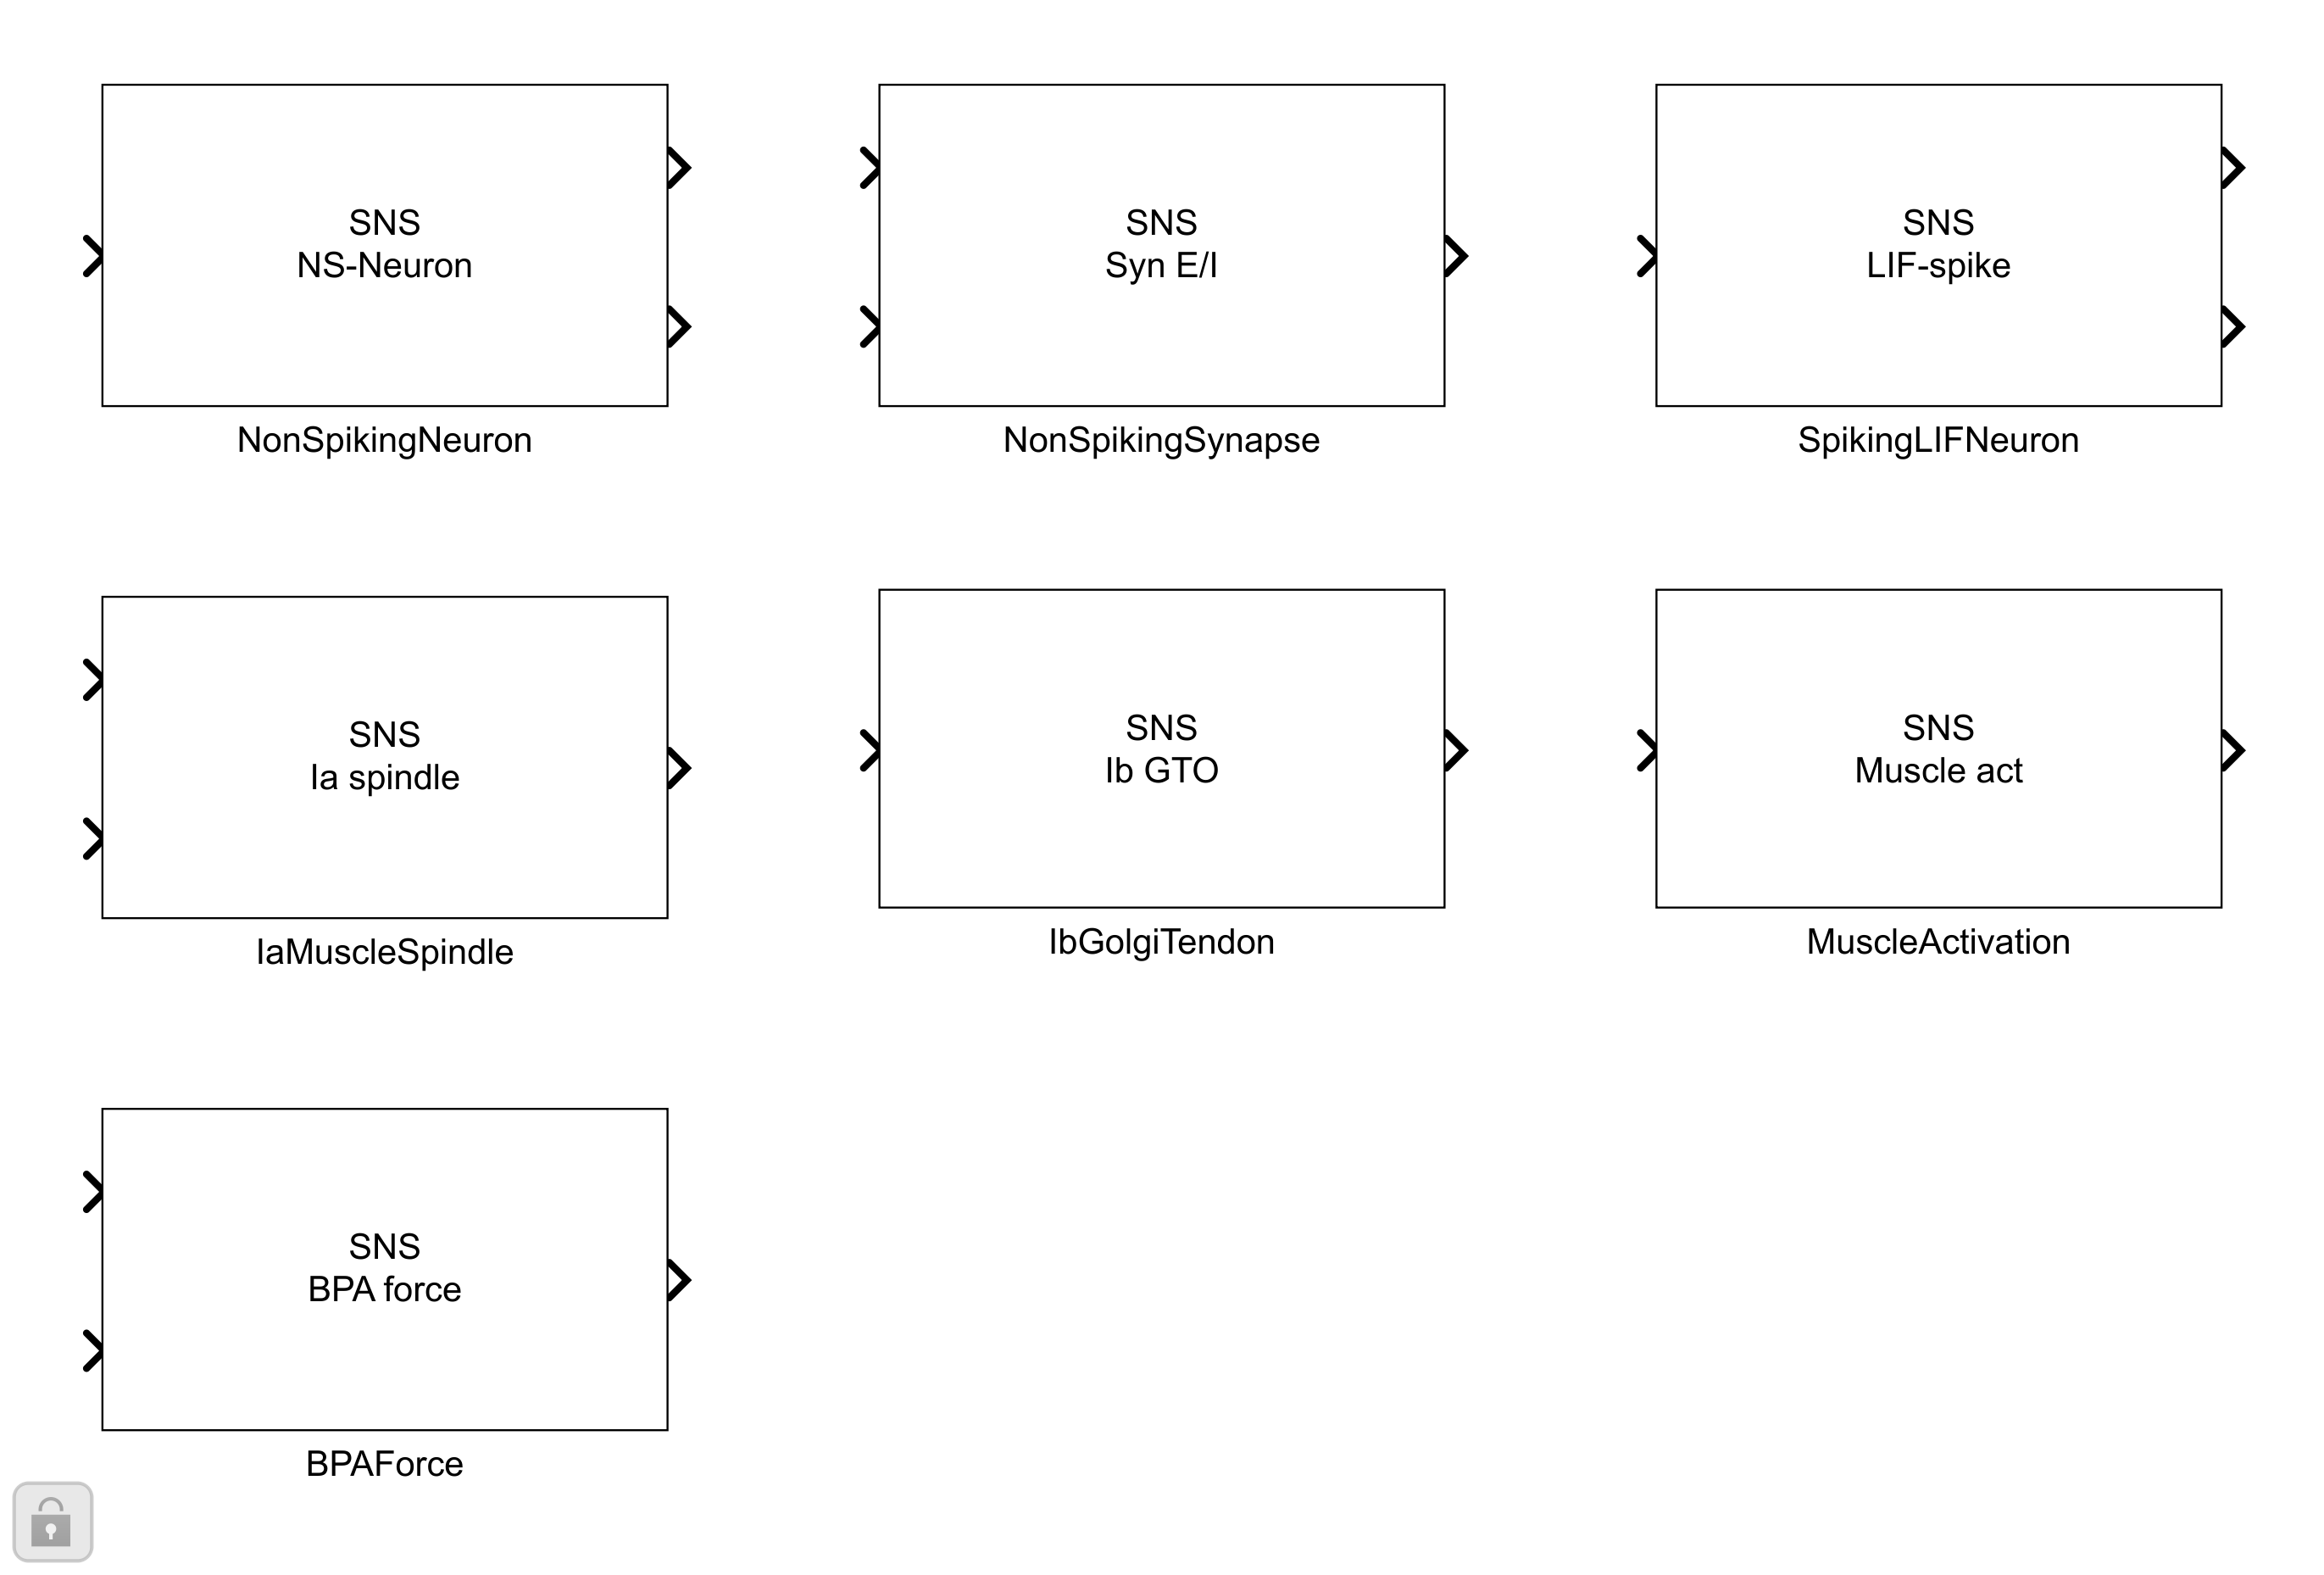
\includegraphics[width=0.95\textwidth,height=0.42\textheight,keepaspectratio]{simulink_sns_library_grid.png}
\par\medskip
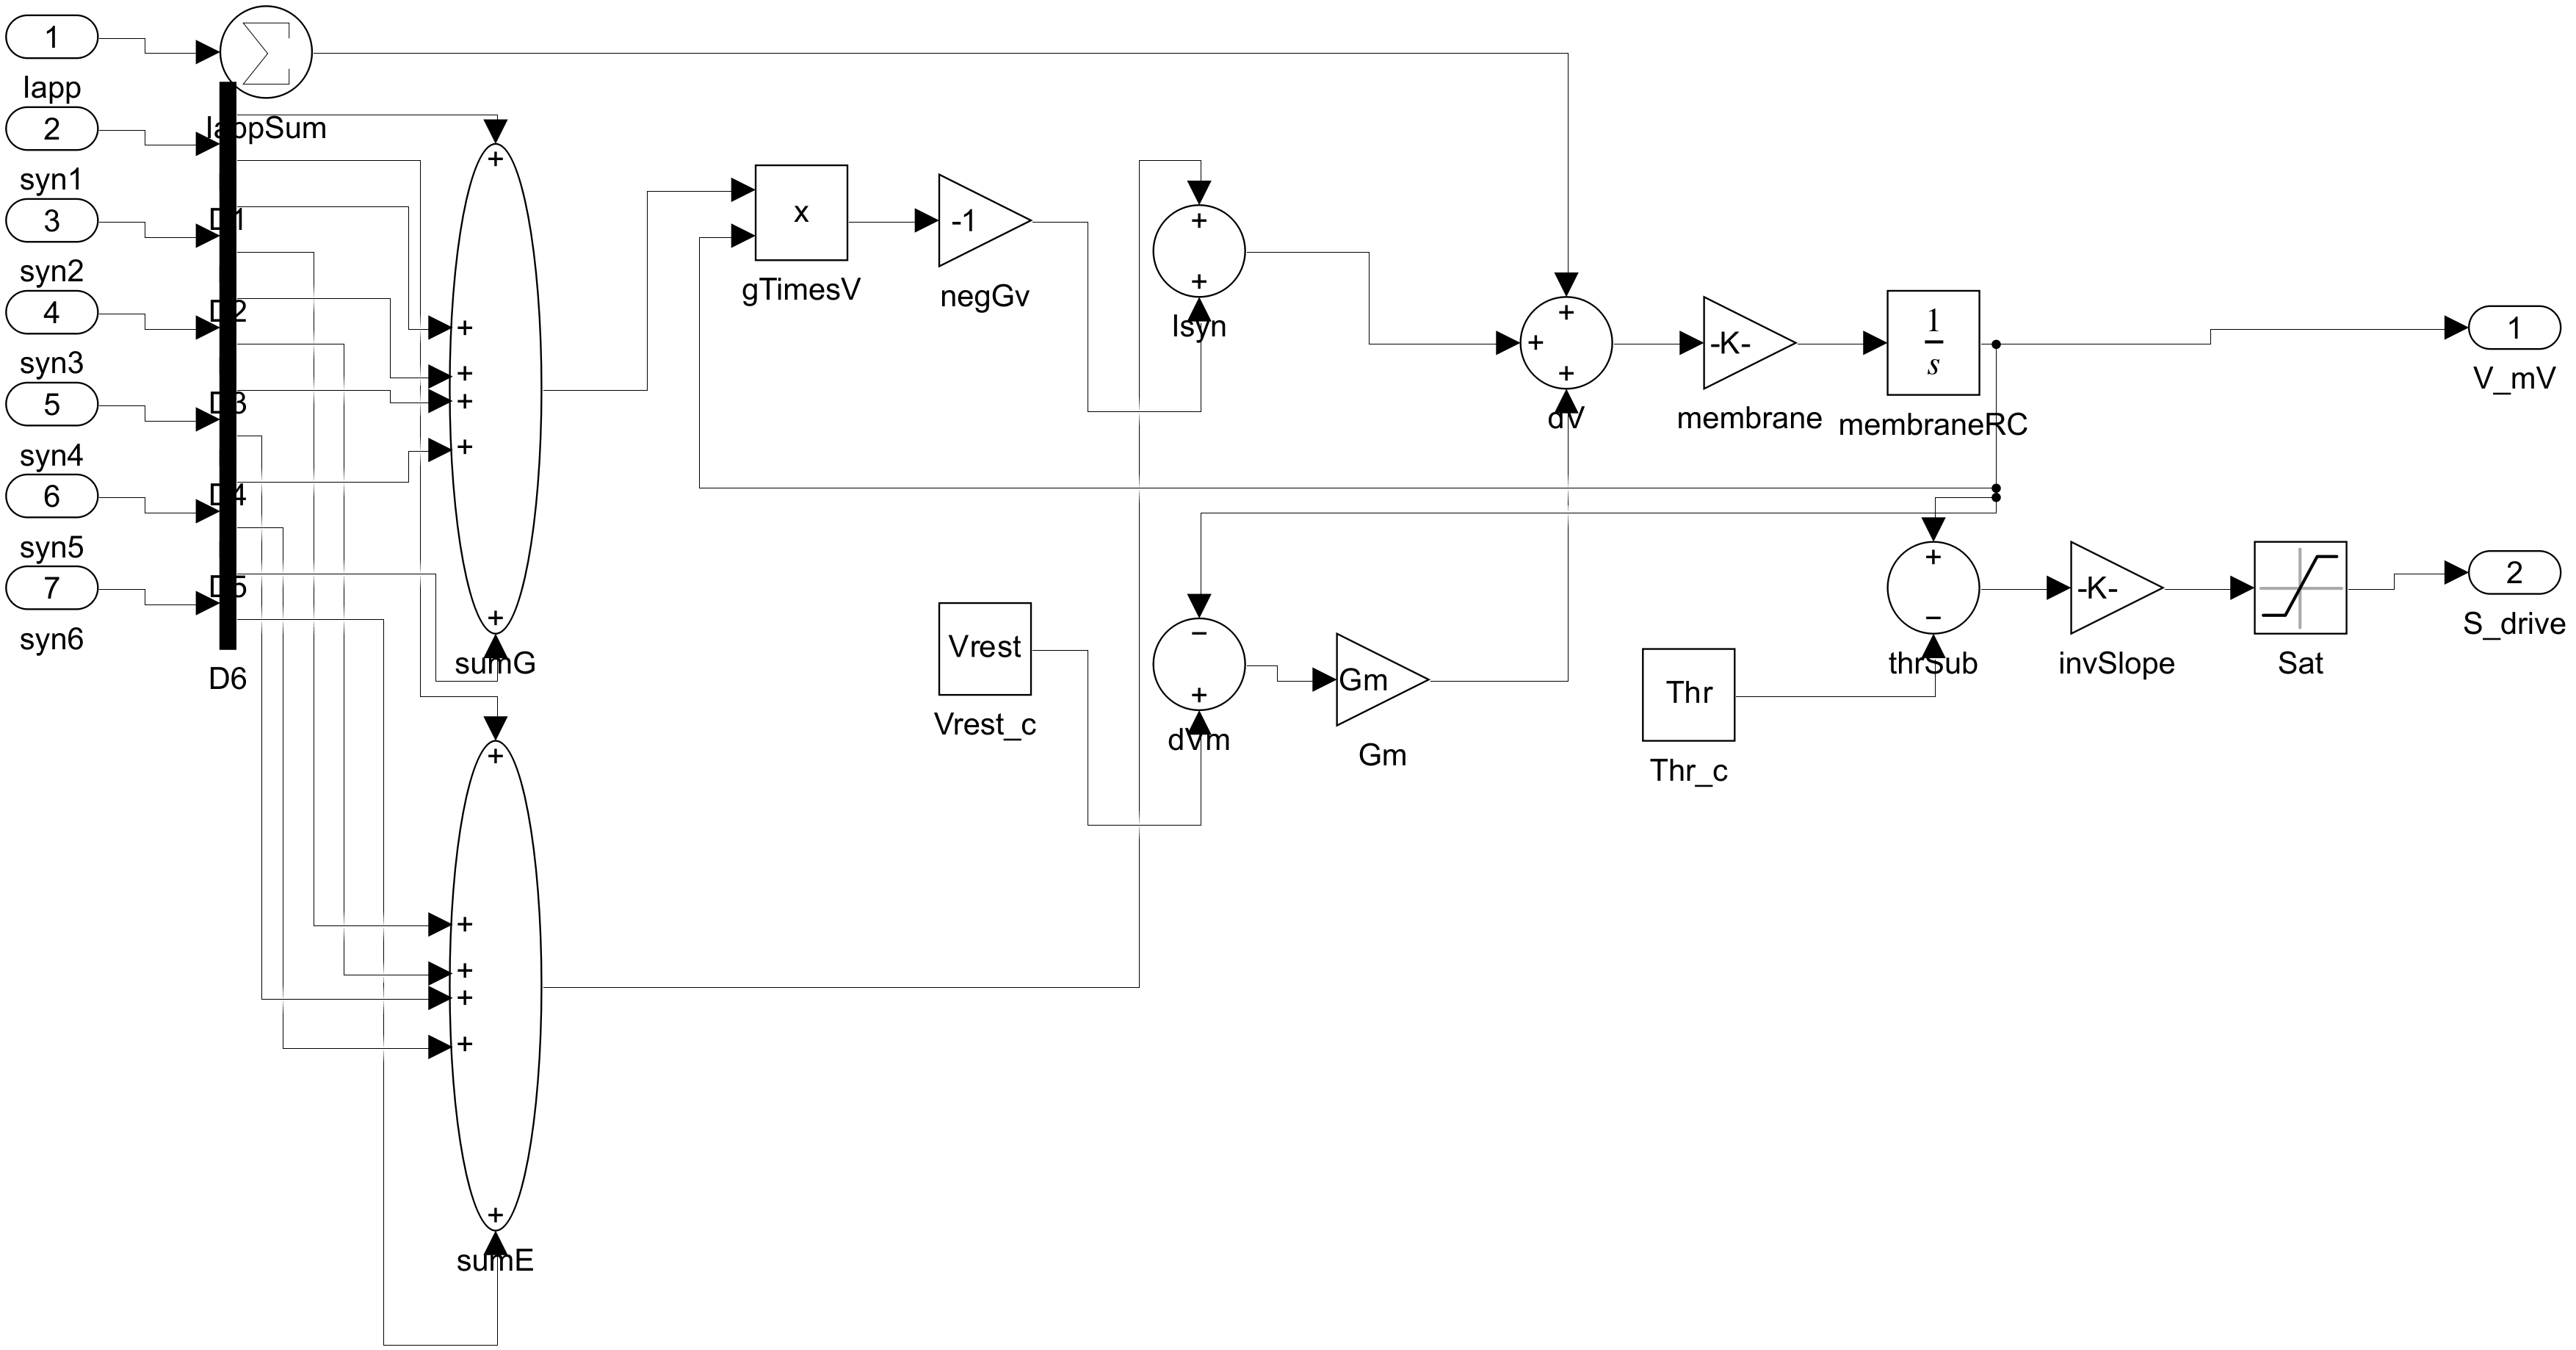
\includegraphics[width=\textwidth,height=0.21\textheight,keepaspectratio]{simulink_neuron_detail.png}
\caption[Simulink SNS library and neuron implementation]{Native Simulink diagram exports showing the seven masked library blocks (top) and the internal implementation of the non-spiking neuron (bottom). The library blocks are arranged in a compact display grid for legibility. The BPA force block remains a placeholder. These implementation views do not establish quantitative knee regulation or a completed CAD-coupled Simscape Multibody model.}
\label{fig:simulink_sns_implementation}
\end{figure}

\begin{sidewaysfigure}[p]
\centering
\includegraphics[width=\textheight,height=0.79\textwidth,keepaspectratio]{simulink_knee_reflex_arranged.png}
\caption[Complete Simulink knee-reflex topology]{The complete reduced-order knee-reflex model exported from Simulink. The diagram connects Ia and Ib sensory pathways, excitatory and inhibitory synapses, antagonist motor neurons, activation and BPA force blocks, and the joint dynamics. Blocks and wires were arranged for display; source and destination ports were checked to confirm unchanged connectivity. Mechanical parameters and the BPA force block remain provisional.}
\label{fig:simulink_reflex_topology}
\end{sidewaysfigure}

\subsection{Cross-Platform Verification of the Contact-Driven Rhythm Core}\label{sec:crossengine_methods}

Because the neuromechanical toolchain assembled here spans several simulation engines, a verification protocol was defined around the contact-driven rhythm core of the two-layer W2L walker architecture: four persistent-sodium half-centers (one extensor/flexor pair per leg) plus graded pattern-formation and sensory cells, driven by heel-contact mechanosensory feedback. The same core was implemented twice from a common connectivity specification --- as a NumPy reference integration through the SNS-Toolbox backend, and as native Simulink blocks from the SNS library of Section~\ref{sec:preliminary_sim_methods} --- and both were driven with an identical protocol: a \qty{12}{\second} run at a \qty{2}{\milli\second} neural step, tonic drive with a brief kickoff pulse, and alternating \qty{1}{\Hz} heel-contact trains. Agreement was scored on rhythm-generator burst period, left--right antiphase correlation, burst counts, and full-trace correlation against the NumPy reference. The archived AnimatLab reference models (the bilateral contact-driven model, the modern W2L model, and the Li walker) were additionally re-run headless from their standalone simulators with instrumented charts, so that engine-level agreement and network-level agreement could be separated. The protocol covers the rhythm core and the archived models only; full-network and whole-body behavior are reported as limitations alongside the results in Section~\ref{sec:preliminary_sim_results}.

% [ZCODE 2026-10-02 Spiking-mirror campaign BEGIN — additive goal-4 dissertation edit. Source of truth: Code/MuJoCo_SNS/spinal/reports_spiking_20261002 (goal1_walkers_spiking.md, goal2_sns_simscape_spiking.md, goal3_animatlab_spiking.md + their artifacts) and Code/MuJoCo_SNS/spinal/SPIKING_MIRROR_PLAN.md. Nothing above this fence was changed.]
\subsection{Spiking-Neuron Mirrors of the Simulation Models}\label{sec:spiking_methods}

The controllers documented above all compute with graded (non-spiking) neurons, in which the membrane potential itself is the analog activity variable that drives the plant. To test that the conclusions drawn from those models are not artifacts of graded coding, spiking-neuron mirrors of all three simulation families were built, following one hybrid doctrine: the motor-neuron layer stays non-spiking, because the musculoskeletal plant consumes a continuous activation command, while the afferent encoders, rhythm-generator half-centers, pattern-formation cells, interneurons, and commissural cells become leaky integrate-and-fire neurons operating at real membrane-potential ranges --- spikes above, analog voltages into the plant \citep{szczecinski_perspective_2023, nourse_sns_2023}. Event-based coding is expected to matter most in the afferent and rhythm layers, where mechanosensor onsets and phase transitions are discrete events, and least at the motor-neuron output, which the muscle activation dynamics low-pass filter anyway.

The MuJoCo--SNS-Toolbox mirror (\texttt{build\_network\_spiking.py}) reproduces the production spinal network of Section~\ref{sec:preliminary_sim_methods} population for population and connection for connection, and is selected at build time by a single environment-variable switch so that the default build path is untouched; that the non-spiking pipeline is unchanged was proven by re-running its defaults gate and baseline evaluation to bit-exact agreement. Because SNS-Toolbox 1.5.2 ships no spiking bursting-neuron class, the rhythm-generator half-centers are adapting integrate-and-fire cells: burst termination is carried by spike-frequency adaptation of the firing threshold, whose time constant reuses the analog network's persistent-sodium inactivation value so that tuned adaptation values transfer between the two builds. Spiking cells rest at \qty{-70}{\mV}, spike at \qty{-50}{\mV}, and reset to \qty{-60}{\mV}, with a tonic bias current parking their equilibrium a few millivolts below threshold --- the analog cells' near-threshold operating point. The network sub-steps at \qty{0.5}{\ms} (four sub-steps inside each \qty{2}{\ms} plant step) so that spike timing is resolved without changing the plant integration, and non-spiking readout taps are appended for the runner's stance gates and neural logging so that all existing analysis code reads analog levels unchanged.

The mirror's synaptic weights are set by a calibration script rather than by hand. Spikes onto the non-spiking motor neurons are calibrated by mean conductance, so that a steady presynaptic train reproduces the non-spiking steady-state motor-neuron voltage (calibration residuals at or below \qty{3e-4}{\mV}); synapses between spiking cells are calibrated by firing-rate transfer (a \qty{40}{\hertz} source drives its target at \qty{40}{\hertz}, and a calibrated inhibitory synapse silences a \qty{40}{\hertz}-driven cell); the graded-to-spiking command pathway is scaled from the measured afferent current-to-rate map. The full calibration of record, with the measured residual of every factor, is tabulated in Appendix~\ref{app:neuron_equations} (Table~\ref{tab:app_spk_cal}).

In the Simulink family, three blocks were added additively to the SNS library of Section~\ref{sec:preliminary_sim_methods} (fifteen blocks at the time of writing): a \texttt{SpikingNeuron} with the same internal synaptic summation as the non-spiking block, an event-wired \texttt{SpikingSynapse} whose conductance jumps by a fixed increment per presynaptic spike and saturates at its maximum, and a \texttt{HybridSpikingSynapse} that carries the same conductance dynamics onto a non-spiking postsynaptic cell. The blocks were verified against the analytic single-spike conductance decay (maximum deviation \qty{6.2e-07}{\micro\siemens}), against a verbatim port of the SNS-Toolbox update equations on a hybrid two-neuron circuit (identical spike count and maximum spike-time deviation \qty{11.75}{\micro\second}), and against the SNS-Toolbox numpy backend itself (mean interspike-interval difference \qty{0.19}{\micro\second}). Spiking twins of the knee-reflex and beverage-holding demonstrations were then built by copy-and-patch: only the sensory interneuron layer and its synapses are replaced by spiking cells, while the motor neurons, muscles, joints, and measurements are identical to the committed demonstrations, and the twin is run at an operating point matched to the baseline gains.

In the AnimatLab family, spiking copies of the runnable standalone exports were produced by scripted conversion of copies, leaving every original file untouched: neuron thresholds are moved from the graded regime (unreachably positive) into the spiking regime, every graded chemical synapse type is re-emitted as a per-spike synapse with the same identity and amplitude (interpreted as a per-spike conductance increment with \qty{10}{\ms} decay), and the per-connection class tag that AnimatLab stores independently of the synapse type is flipped to match. A calibrated variant sets each cell class's threshold just below its measured graded peak, and an ablation that converts the thresholds but keeps the graded synapses isolates which change does what. Each copy passes a structural validator (neuron, connection, synapse-type, chart, and stimulus sets identical to its original, and every class tag consistent) and runs headless to its configured end. The 2023 spiking walker model of the same lineage, which was tuned as a rate code from birth, serves as the spiking reference baseline for this family.

Each mirror is verified against its non-spiking twin by a fixed gate set rather than by inspection: a topology gate requires the connection multiset to be identical between the two builds under three gain configurations; a rhythm gate requires self-sustained alternating rhythm under constant drive with the period within \qty{20}{\percent} of the analog build; a basin gate requires the rhythm to persist under \qty{1}{\percent} multiplicative jitter on every scalar parameter; an air-regime smoke gate compares cadence, duty, and joint ranges of the deafferented suspended-air preparation; and a regression gate requires every committed non-spiking artifact to reproduce its recorded values exactly with the spiking blocks present in the library. The mirrors carry mapped parameters only --- no new tuning was performed --- so their results (Section~\ref{sec:spiking_results}) establish what transfers structurally and what requires re-tuning, and any fresh tuning campaign is future work.
% [ZCODE 2026-10-02 Spiking-mirror campaign END]

\section{Preliminary Neuromechanical Simulation Recordings}\label{sec:preliminary_sim_results}

The AnimatLab phase-1 run described in Section~\ref{sec:preliminary_sim_methods} produced synchronized joint, neural, contact-sensory, and body-motion recordings over \qty{10}{\second}. Basic checks confirmed finite values and a uniform \qty{0.2}{\milli\second} sampling interval in both exported charts. Each chart contained 50,001 samples from 0 through \qty{10}{\second}; nine trailing zero-filled rows beyond the configured chart end were excluded. Figure~\ref{fig:animatlab_phase1_preliminary} shows bilateral hip, knee, and ankle angles. Neural and contact-sensory recordings remain archived with the run; the contact-sensory channels record membrane voltage rather than contact force. These recordings demonstrate signal acquisition and alternating activity in this run, rather than validated locomotor performance. The model included an externally applied horizontal force during the first second, and neither stable walking nor effective ground-contact gating was established.

\begin{figure}[htbp]
\centering
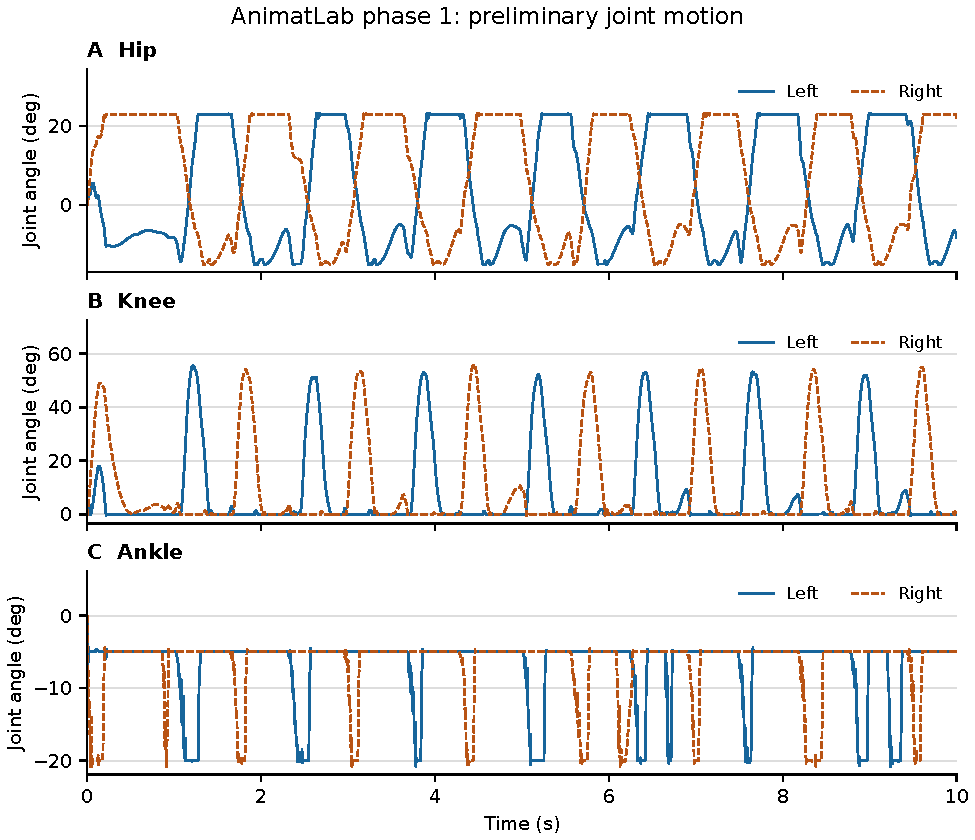
\includegraphics[width=\textwidth,height=0.60\textheight,keepaspectratio]{animatlab_phase1_joint_angles.pdf}
\caption[Preliminary AnimatLab hip, knee, and ankle recordings]{Preliminary AnimatLab phase-1 joint motion: \textbf{(A)} hip, \textbf{(B)} knee, and \textbf{(C)} ankle angles in the model's recorded joint conventions. Blue solid and orange dashed traces denote left and right sides. All 50,001 samples within the configured 0--\qty{10}{\second} chart window are retained without filtering. The model includes an external horizontal force during the first second. These traces document joint motion in an instrumented run; they do not establish stable walking or effective ground-contact gating.}
\label{fig:animatlab_phase1_preliminary}
\end{figure}

\subsection{Cross-Engine Verification of the Contact-Driven Rhythm Core}\label{sec:crossengine_results}

The verification protocol of Section~\ref{sec:crossengine_methods} was applied to the W2L rhythm core. Between the NumPy reference and the native Simulink reimplementation, both legs' rhythm-generator burst periods matched at \qty{1.000}{\second} versus \qty{1.000}{\second} (0.0\% error), the left--right antiphase correlation reproduced the reference exactly ($r = -0.525$), and all ten expected bursts occurred in the scored window. The full voltage traces cross-correlate at $r = 0.99996$--$0.99998$ at a $-\qty{2}{\milli\second}$ lag with an RMSE of 0.099--0.111~mV (Figure~\ref{fig:w2l_crossengine}); the residual lag is consistent with the one-step delay of the discrete Simulink solver. The same protocol surfaced an architectural fact rather than a defect: with the heel-contact trains removed, the full network holds a static latch under tonic drive with kickoff alone, in every implementation --- so phasic contact feedback is part of the drive architecture of the W2L design, not an optional perturbation.

\begin{figure}[htbp]
\centering
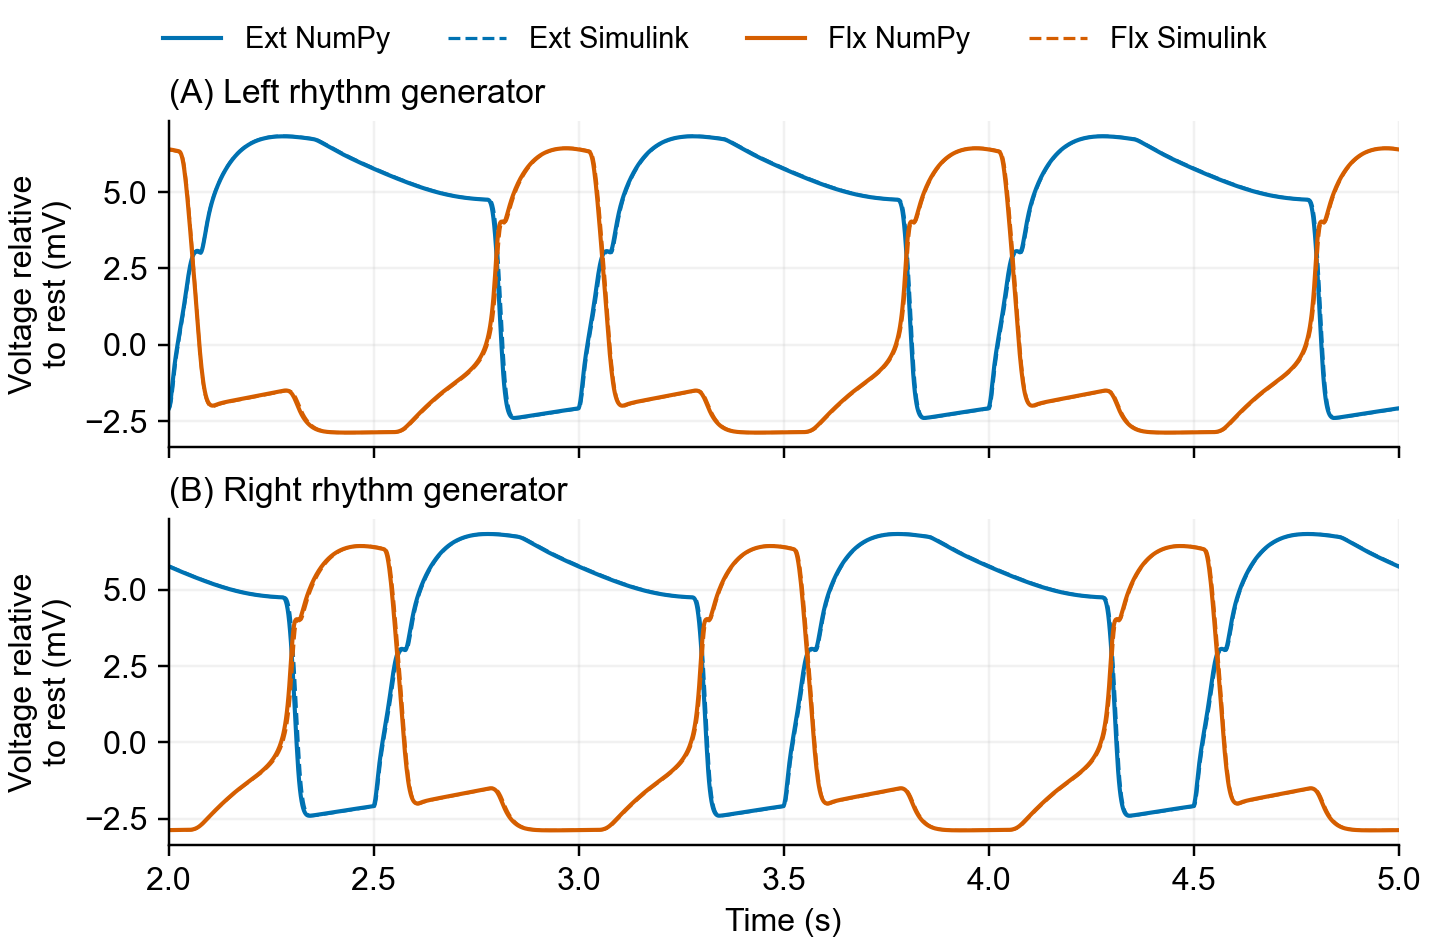
\includegraphics[width=\textwidth,height=0.55\textheight,keepaspectratio]{sns_w2l_traces.png}
\caption[W2L rhythm-core traces across engines]{Left and right rhythm-generator extensor half-center voltages of the W2L contact-driven rhythm core under the shared verification protocol, from the NumPy reference (SNS-Toolbox backend) and the native Simulink reimplementation. Scored metrics --- burst period, left--right antiphase correlation, and burst counts --- agree exactly, and the full traces cross-correlate at $r \geq 0.99996$ at a $-\qty{2}{\milli\second}$ lag.}
\label{fig:w2l_crossengine}
\end{figure}

\subsection{Headless Validation of the AnimatLab Reference Models}\label{sec:animatlab_validation}

The archived AnimatLab reference models were re-run headless from their standalone simulators with instrumented charts, and eleven targetable rhythm and gait metrics were extracted automatically; all eleven pass their acceptance bands. In the bilateral contact-driven model, the rhythm generators oscillate at periods of \qty{0.450}{\second} (left) and \qty{0.467}{\second} (right) with a left--right lag of \qty{0.529}{cycle} (cross-correlation $r = 0.976$), confirming alternating gait timing. In the modern W2L model, the joints oscillate at \qty{2.25}{\Hz}; its flexor half-centers peak at $-\qty{56.4}{\mV}$ and never cross the $-\qty{55}{\mV}$ threshold, so the rhythm is carried by clean extensor/flexor antiphase ($r = -0.996$) through the graded pathway rather than by flexor spiking. The Li-model rerun \citep{li_bipedal_2017} walks at \qty{0.637}{\meter\per\second} with right and left step periods of \qty{1.299 \pm 0.024}{\second} and \qty{1.333 \pm 0.080}{\second} and duty factors of 0.443 and 0.555, reproducing the published behavior of the original model in its original engine.

\subsection{BPA-Actuated Walker in MuJoCo}\label{sec:bpa_walker}

The walker geometry of Section~\ref{sec:prior_walker} was exported to MuJoCo and driven by antagonistic BPA actuator pairs under the split contact-driven network, with actuator forces computed by the BPA model of Chapter~\ref{ch:methods}. In the air-stepping gate --- the harness carrying 70\% of the \qty{411}{\N} body weight --- the walker produced clean knee-flexion excursions at a \qty{1.542}{\second} period with a knee flexion range of \ang{63.5}, peak BPA forces of \qty{880}{\N} (left) and \qty{1372}{\N} (right) at a peak pressure of \qty{372}{\kPa} --- 60\% of the \qty{620}{\kPa} ceiling --- and 7 and 5 heel-contact episodes on the left and right. This run demonstrates the complete chain from the characterized BPA force model to a multi-joint walker stepping under synthetic neural control, with actuator sizing operating inside the characterized pressure range.

The same campaign reported its failures with equal weight. On the ground, the W2L gate model stands (full-support stance) but does not walk: heel duty is zero and forward displacement is $+\qty{0.001}{\meter}$ over the run. The MuJoCo port of the Li model produced no stance episodes in any of seven drop-protocol variants. Together with the latch result of Section~\ref{sec:crossengine_results}, these negatives localize the open problem precisely: the contact-driven rhythm architecture itself transfers across engines intact, but translating it to unsupported ground locomotion requires the balance and weight-bearing layers defined in Chapter~\ref{ch:futurework}, and those layers are not present in these models.

% [ZCODE 2026-10-03 Walker-validation sweep subsections BEGIN: additive edit anchored after the closing paragraph of Section~\ref{sec:bpa_walker}, immediately before the 2026-10-02 spiking fence (which was not touched). Numbers from the 2026-10-03 session digest only (gait_validation_20260930.csv, prune_results_{s3k,syn6,w2lvar}.jsonl, robust_results_{s3k,s3kpruned,syn6,w2lvar}.jsonl). Score convention per kine_ref.py: higher is better, 0 = perfect, -25 = fixed no-cycle fallback (runner.py).]
\subsection{Gait-Validation Sweep against the Locomotion Reference Library}\label{sec:gait_library_results}

The four production walking configurations of the converted robot-body model were evaluated against a library of 43 human locomotion reference cycles: 32 running trials from eight subjects at four speeds, ten walking references (seven at prescribed speeds from \qty{0.5}{\metre\per\second} to \qty{2.0}{\metre\per\second}, plus three self-selected), and one further reference cycle, \texttt{Case\_40\_motion}, the predicted-walking cycle of the Falisse predictive-simulation dataset (period \qty{1.11}{\second}, duty factor 0.57). The four configurations span the two controller lineages of this program. The human-derived lineage contributes the production walking configuration (\texttt{s3k}), whose two-level network was tuned against the human walking reference, its pruned derivative (\texttt{s3kpruned}), and the six-synergy variant (\texttt{syn6}), whose pattern-formation layers drive the motor pools through a six-synergy basis extracted from human gait data. The robot-walker lineage contributes the W2L-layout variant (\texttt{w2lvar}), which restructures the rhythm and pattern-formation layers after the contact-driven W2L circuit of Section~\ref{sec:crossengine_methods}. Each configuration was scored with the production pipeline's cycle-shape kinematic score, in which 0 denotes perfect agreement and $-25$ is the fixed no-cycle fallback, both on its tuning-reference evaluation and against every library cycle (Table~\ref{tab:gait_sweep}).

\begin{table}[htbp]
\caption{Gait-validation sweep of the four production walking configurations against the 43-cycle locomotion reference library. The score is the production pipeline's cycle-shape kinematic score (0 denotes perfect agreement); the tuning-reference score is each configuration's evaluation on the tuning pipeline's walking reference, and the library mean averages the same score over all 43 references (among genuine gait cycles, higher scores indicate closer agreement).}
\label{tab:gait_sweep}
\begin{tabular}{@{}lrrl@{}}
\toprule
 & \textbf{Tuning-ref.} & \textbf{Library mean} & \textbf{Most negative reference} \\
 & \textbf{score} & \textbf{score (43 refs)} & \textbf{(score)} \\
\midrule
\texttt{s3k}        & $-186.4$ & $-8776$ & \texttt{Case\_40\_motion} ($-8841$) \\
\texttt{s3kpruned}  & $-176.1$ & $-6924$ & \texttt{Case\_40\_motion} ($-6986$) \\
\texttt{syn6}       & $-200.4$ & $-9961$ & \texttt{Case\_40\_motion} ($-10040$) \\
\texttt{w2lvar}     & $-144.5$ & $-5808$ & \texttt{subject08\_Run\_20002} ($-5896$) \\
\bottomrule
\end{tabular}
\end{table}

The ranking is identical in the two evaluations: the W2L-layout variant agrees most closely with both its tuning reference and the library on average (\texttt{w2lvar} at $-144.5$ and $-5808$), the six-synergy variant least closely (\texttt{syn6} at $-200.4$ and $-9961$), and the two production configurations fall between, with pruning moving \texttt{s3k} toward closer agreement ($-186.4$ and $-8776$ for \texttt{s3k}, against $-176.1$ and $-6924$ for \texttt{s3kpruned}). Every configuration's library scores are one to two orders of magnitude more negative than its tuning-reference score, which quantifies how far a network tuned to a single walking reference transfers to the library's diverse reference cycles; the gap is not an artifact of the 32 running trials, because the production configuration's mean over the ten walking references alone ($-8816$) is slightly more negative than its running-only mean ($-8761$) and essentially its overall library mean ($-8776$). The most negative single score for three of the four configurations falls on the same library reference, \texttt{Case\_40\_motion} ($-8841$ for \texttt{s3k}, $-6986$ for \texttt{s3kpruned}, and $-10040$ for \texttt{syn6}), while the W2L-layout variant's most negative reference is a running trial, \texttt{subject08\_Run\_20002} ($-5896$). All four configurations produce right-leg-only or asymmetric gait in these evaluations. At the family level, the sweep's reading is that the robot-walker-lineage configuration, not the human-derived ones, agrees most closely with the library, while the six-synergy configuration, the most strongly human-derived in its pattern formation, agrees least closely.

\subsection{Comparison of the Production Walker Variants}\label{sec:walker_variant_results}

The same campaign removed individual pathway classes from each configuration and re-evaluated the tuning-reference score, identifying which pathways each lineage depends on (Table~\ref{tab:walker_ablations}). In the production configuration, removing the Ia afferent pathway freezes the model outright: the evaluation detects no gait cycles and returns the fixed $-25$ fallback. Removing the Renshaw cells, the group-II afferents, or all afferent classes at once degrades the score to $-267.3$, $-255.2$, and $-267.8$, respectively, against the full model's $-186.4$, while removing the Ib, contact, or interleg commissural channels individually shifts the score by smaller amounts toward zero ($-180.3$, $-183.9$, and $-174.9$). The six-synergy variant behaves differently: with all afferents removed it scores $-190.5$ against its full model's $-200.4$ and still walks bilaterally, with ten cycles on each leg, a knee-flexion minimum of \ang{-71.2}, and a \qty{0.684}{\second} period, so its afferent complement is not what sustains its gait. The W2L-layout variant depends on both the Ia pathway (removed: $-273.5$) and the weak rhythm-generator mutual excitation (removed: $-279.9$) against its full model's $-144.5$ with four right-leg and six left-leg cycles, while removing its Renshaw cells leaves a bilateral gait at $-142.4$.

\begin{table}[htbp]
\caption{Pathway-removal sweep on the tuning-reference evaluation. The score is the production pipeline's cycle-shape kinematic score (0 denotes perfect agreement; $-25$ is the fixed no-cycle fallback, a failed evaluation that scores above every genuine gait in this table). The full-model rows repeat each configuration's unmodified production evaluation.}
\label{tab:walker_ablations}
\begin{tabular}{@{}llr@{}}
\toprule
\textbf{Configuration} & \textbf{Removed pathway} & \textbf{Score} \\
\midrule
\texttt{s3k} (full model) & none & $-186.4$ \\
 & Ia afferents & $-25$ (no cycles detected) \\
 & all afferent classes & $-267.8$ \\
 & Renshaw cells & $-267.3$ \\
 & group-II afferents & $-255.2$ \\
 & Ib afferents & $-180.3$ \\
 & contact channels & $-183.9$ \\
 & interleg commissural pathways & $-174.9$ \\
\addlinespace
\texttt{syn6} (full model) & none & $-200.4$ \\
 & all afferent classes & $-190.5$ \\
\addlinespace
\texttt{w2lvar} (full model) & none & $-144.5$ \\
 & Ia afferents & $-273.5$ \\
 & weak rhythm-generator mutual excitation & $-279.9$ \\
 & Renshaw cells & $-142.4$ \\
\bottomrule
\end{tabular}
\end{table}

Drive-perturbation and push testing splits the field along family lines. The production configuration never fell in 15 stand and push evaluations (maximum push sway \qty{0.123}{\meter}), and its walk survives drive perturbations of $+0.01$, $-0.01$, and $-0.02$ (scores of $-201.9$, $-177.0$, and $-171.2$), freezing only at $+0.02$; its pruned derivative survives the unperturbed evaluation ($-176.1$) and the $-0.02$ perturbation ($-168.2$). The six-synergy and W2L-layout variants fall under every $\pm 0.01$ and $\pm 0.02$ drive perturbation tested, with pelvis tilt reaching \ang{39} to \ang{40}. The sweep therefore identifies the production configuration and its pruned derivative as the robust pair of the family, and locates the fragility of the six-synergy and W2L-layout variants under drive perturbation.
% [ZCODE 2026-10-03 Walker-validation sweep subsections END]

% [ZCODE 2026-10-02 Spiking-mirror campaign BEGIN — additive goal-4 dissertation edit. Source of truth: Code/MuJoCo_SNS/spinal/reports_spiking_20261002 (goal1/goal2/goal3 reports + artifacts; supervisor-gated campaign). Methods: Section~\ref{sec:spiking_methods}; full tables in Appendix~\ref{app:neuron_equations}. Nothing above this fence was changed.]
\section{Spiking-Neuron Mirror Results}\label{sec:spiking_results}

The spiking-neuron mirrors of Section~\ref{sec:spiking_methods} were evaluated against their non-spiking twins in the same order in which the families were introduced: the MuJoCo spinal network, the Simulink demonstrations, and the AnimatLab walker family. All numbers in this section come from the gated verification campaign whose artifacts and reproduction commands are catalogued in Appendix~\ref{app:neuron_equations}.

\subsection{MuJoCo Spinal-Network Mirror}

The non-spiking production baselines were first re-established on the machine of record: all three current production configurations reproduce their documented evaluation scores exactly, including the default build's kinematic score of $-161.56754173676563$, and after the mirror's selector was added the default build gate ($(410, 376, 1186)$ populations, inputs, and connections) and that same baseline score reproduce digit for digit, proving the non-spiking pipeline untouched.

The topology gate passes exactly: under the default, fully tuned, and joint-layer pattern-formation gain configurations, the spiking mirror's directed connection multiset is identical to the non-spiking build's ($1{,}186$, $7{,}908$, and $7{,}762$ connections respectively), with identical input lists, identical motor-neuron maps, and exactly the expected number of readout taps (12, 12, and 16). The mirror is structurally the same network.

Under constant drive (network alone, \qty{20}{\second}), the rhythm gate splits. The spiking mirror self-sustains clean bilateral antiphase --- rhythm-generator extensor and flexor cells firing at \qty{4.9}{\hertz} and \qty{3.2}{\hertz} per leg, with the swing readout sustained in every window --- but its envelope period is \qty{0.621}{\second} against the analog build's \qty{0.399}{\second}, a \qty{55.6}{\percent} lengthening that misses the gate's \qty{20}{\percent} tolerance (Figure~\ref{fig:spike_rhythm}). The basin gate passes in full: the rhythm persists under \qty{1}{\percent} multiplicative jitter on every scalar parameter in all 12 seeded trials, with a final-window swing minimum of \qty{4.58}{\mV} against the \qty{5.13}{\mV} baseline (margin $0.89\times$) and no divergent trials. In the deafferented suspended-air preparation, the mirror air-steps rhythmically with full-amplitude joint swings (knee range \ang{106.0} against the twin's \ang{117.9}), but its cadence is roughly ten times faster than the non-spiking twin's \qty{0.47}{\hertz} air-stepping regime in this preparation, so the air-regime gate fails on the cadence clause alone.

\begin{figure}[htbp]
\centering
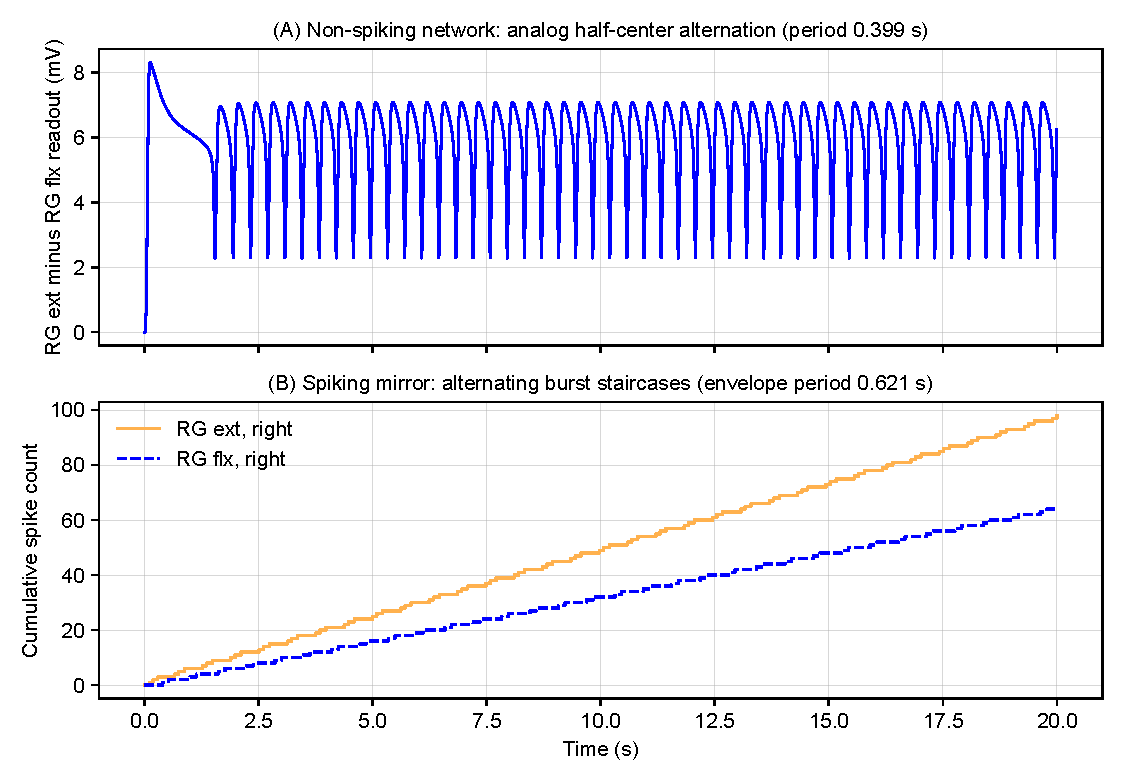
\includegraphics[width=\textwidth]{spiking_mirror_rhythm.pdf}
% ALT TEXT: see spiking_mirror_rhythm_alt.txt beside the figure file.
\caption[Constant-drive rhythm, non-spiking versus spiking]{Constant-drive rhythm of the right rhythm-generator under network-only simulation. \textbf{(A)} The non-spiking network's extensor-minus-flexor readout voltage alternates irregularly about a \qty{4.8}{\milli\volt} swing (larger only in the startup transient), with an average period of \qty{0.399}{\second}. \textbf{(B)} The spiking mirror's raw extensor (solid orange) and flexor (dashed indigo) cells fire in alternating bursts whose envelope period is \qty{0.621}{\second}, \qty{55.6}{\percent} longer than the analog build.}
\label{fig:spike_rhythm}
\end{figure}

One untuned ground-walking evaluation was run as a stretch attempt: the spiking mirror at the non-spiking winner's mapped parameters, with no re-tuning. It scores worse overall (kinematic score $-236.35$ against $-161.57$), as expected for an untuned mapped starting point, but it produces a genuine bilateral gait --- eight right-leg and nine left-leg cycles, a cycle-window knee flexion minimum of \ang{-79.8}, no non-finite states, and the model stays up --- whereas the non-spiking winner's left leg is frozen (zero cycles) in every recorded run of its study, including this session's baseline (Figure~\ref{fig:spike_ground}, Table~\ref{tab:spike_ground}). This is a single run with no statistics, reported as a lead for the fresh tuning campaign that the mirror's plan calls for, not as an established gait result.

\begin{table}[htbp]
\caption{Untuned spiking mirror versus its non-spiking twin at the same winner parameters, ground evaluation (16 s). The cycle knee minimum and stance fractions are computed over detected gait cycles; the kinematic score is the cycle-shape error metric of the production pipeline (0 denotes perfect agreement; higher scores indicate closer agreement). The spiking mirror carries mapped parameters only, with zero re-tuning.}
\label{tab:spike_ground}
\begin{tabular}{@{}lcc@{}}
\toprule
\textbf{Metric} & \textbf{Non-spiking winner} & \textbf{Spiking mirror (untuned)} \\
\midrule
Kinematic score                & $-161.57$          & $-236.35$ \\
Gait cycles, right / left      & 9 / 0 (left frozen) & 8 / 9 (bilateral) \\
Cycle knee minimum             & \ang{-64.3}         & \ang{-79.8} \\
Contact duty, right / left     & 0.637 / 0.985       & 0.799 / 0.856 \\
Maximum pelvis tilt            & \ang{22.1}          & \ang{19.2} \\
Non-finite states / fell       & no / up             & no / up \\
\bottomrule
\end{tabular}
\end{table}

\begin{figure}[htbp]
\centering
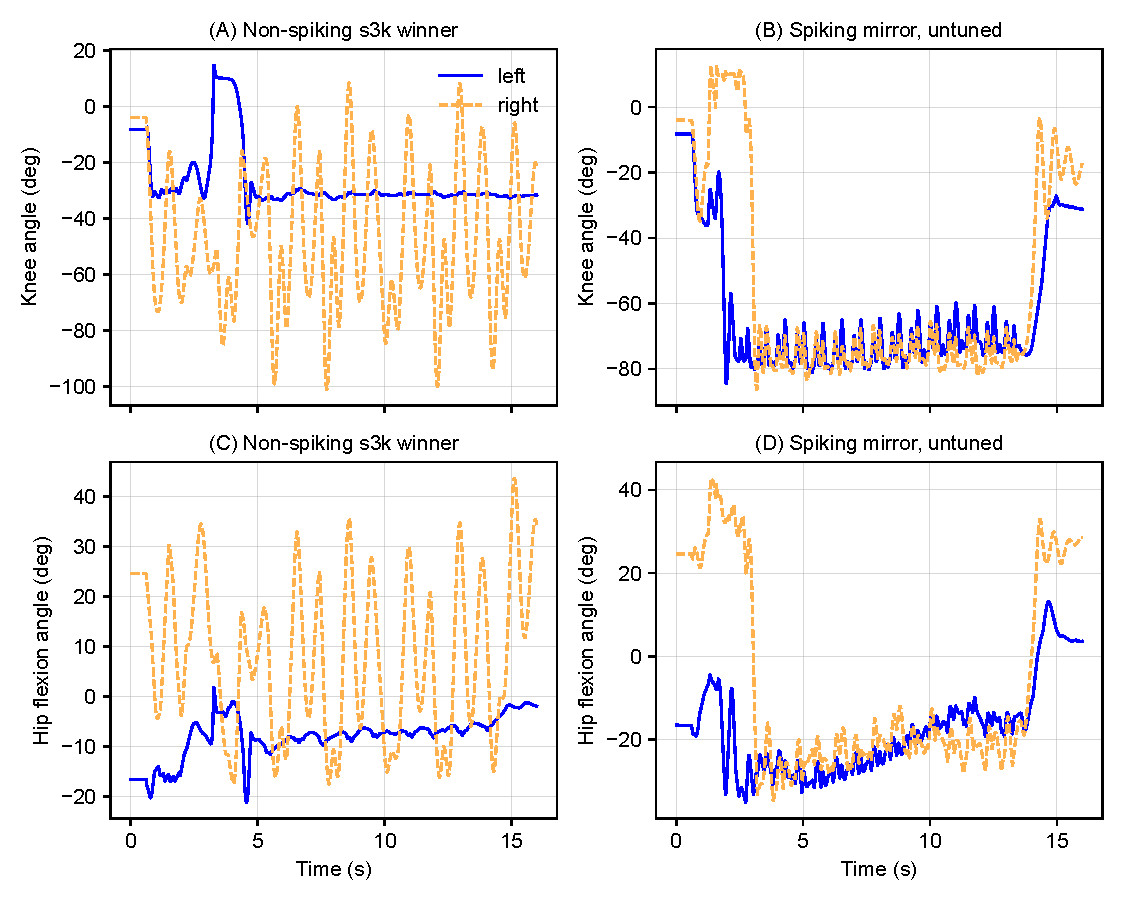
\includegraphics[width=\textwidth]{spiking_mirror_ground_gait.pdf}
% ALT TEXT: see spiking_mirror_ground_gait_alt.txt beside the figure file.
\caption[Ground gait, non-spiking winner versus untuned spiking mirror]{Ground-walking joint angles of the converted MuJoCo robot at the non-spiking winner's parameters. \textbf{(A, C)} The non-spiking winner steps with the right leg only; the left knee moves through a single slow excursion without cycling. \textbf{(B, D)} The untuned spiking mirror cycles both legs with deep knee flexion. Solid indigo traces denote the left leg, and dashed orange traces denote the right leg.}
\label{fig:spike_ground}
\end{figure}

\subsection{Simulink Spiking Demonstration Twins}

The three new library blocks were verified at the unit level before any demonstration was rebuilt. The single-spike conductance transient matches the exact exponential to \qty{6.2e-07}{\micro\siemens}, saturating pulse-train accumulation matches to \qty{4.6e-05}{\micro\siemens}, and a hybrid two-neuron circuit matches a verbatim port of the SNS-Toolbox update equations spike for spike (62 of 62 spikes, maximum spike-time deviation \qty{11.75}{\micro\second}, maximum voltage deviation \qty{1.2e-02}{\mV}). The same circuit run through the SNS-Toolbox numpy backend agrees with the Simulink copy to \qty{0.19}{\micro\second} in mean interspike interval and \qty{0.81}{\micro\volt} in final voltage. With the spiking blocks present in the library, every committed demonstration and units test reproduces its recorded value exactly, including the committed two-neuron units test at \qty{6.07e-04}{\mV}.

At the matched operating point, the spiking twin of the knee-reflex demonstration is indistinguishable from the baseline in its transient and within one degree in its settle behavior (Table~\ref{tab:spike_knee}, Figure~\ref{fig:spike_knee}): both read \ang{15.79} at \qty{0.05}{\second}, and the twin settles \ang{0.9} higher with a slightly hotter, faster antagonist alternation, because the rate-coded pathway adds the synaptic filter time constant that graded synapses do not have. The spiking twin of the beverage-holding demonstration likewise holds the cup at essentially the same level, with the reflex-off sag identical to the baseline and the reflex modulation within \ang{0.02} (Table~\ref{tab:spike_beer}).

\begin{table}[htbp]
\caption{Knee-reflex demonstration, committed baseline versus spiking twin at the matched operating point (5 s runs; settle statistics over the last \qty{2}{\second}).}
\label{tab:spike_knee}
\begin{tabular}{@{}lcc@{}}
\toprule
\textbf{Metric} & \textbf{Baseline} & \textbf{Spiking twin} \\
\midrule
Knee angle at \qty{0.05}{\second}   & \ang{15.79} & \ang{15.79} \\
Settle mean (last \qty{2}{\second}) & \ang{43.5}  & \ang{44.4} \\
Settle range                        & \ang{41.6}--\ang{44.9} & \ang{41.9}--\ang{46.7} \\
Extensor / flexor activation (window means) & 0.53 / 0.53 & 0.58 / 0.56 \\
Antagonist alternation              & \qty{0.5}{\hertz}--\qty{2}{\hertz} & \qty{7.4}{\hertz} (dominant peak) \\
Ia interneuron firing at settle     & graded, subthreshold & \qty{95}{\hertz}; Ib \qty{0}{\hertz} \\
\bottomrule
\end{tabular}
\end{table}

\begin{table}[htbp]
\caption{Beverage-holding demonstration, committed baseline versus spiking twin (10 s pour; sag measured after \qty{2}{\second}).}
\label{tab:spike_beer}
\begin{tabular}{@{}lcc@{}}
\toprule
\textbf{Metric} & \textbf{Baseline} & \textbf{Spiking twin} \\
\midrule
Maximum sag, reflex on             & \ang{2.00} & \ang{2.02} \\
Maximum sag, reflex off            & \ang{7.85} & \ang{7.85} \\
Reflex modulation (off minus on)   & \ang{5.85} & \ang{5.83} \\
Biceps activation over the pour    & 0.392 $\to$ 0.417 & 0.392 $\to$ 0.447 \\
Triceps activation over the pour   & 0.400 $\to$ 0.316 & 0.400 $\to$ 0.254 \\
Biceps Ia firing rate (reflex on)  & graded     & \qty{166.6}{\hertz} (mean) \\
\bottomrule
\end{tabular}
\end{table}

\begin{figure}[htbp]
\centering
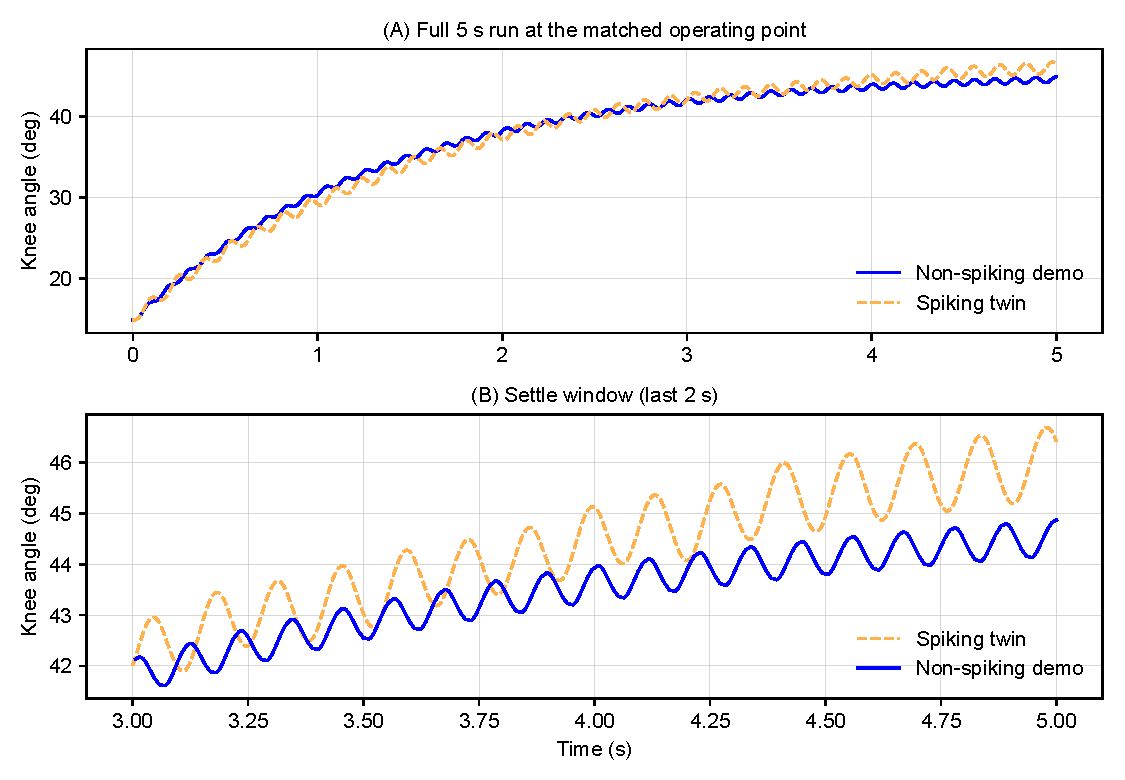
\includegraphics[width=\textwidth]{simulink_knee_spiking_twin.pdf}
% ALT TEXT: see simulink_knee_spiking_twin_alt.txt beside the figure file.
\caption[Simulink knee-reflex twin, baseline versus spiking]{Knee angle of the Simulink knee-reflex demonstration: committed non-spiking baseline (solid indigo) versus spiking twin (dashed orange) at the matched operating point. \textbf{(A)} Full \qty{5}{\second} run. \textbf{(B)} Settle window (last \qty{2}{\second}); the spiking twin's alternation band is slightly wider.}
\label{fig:spike_knee}
\end{figure}

A representative rhythm-generator-to-motor-pool subnetwork demonstrates the hybrid motif end to end: spiking half-centers with laminated inhibition drive a non-spiking three-motor-neuron pool whose voltage stays graded over a \qty{5}{\milli\volt} depth ($-52.0$ to $-46.9$~mV) and tracks its rhythm generator's rate envelope. Burst alternation in that subnetwork is partial --- the extensor half-center bursts four times in \qty{12}{\second} while the flexor half-center keeps a low-rate floor through the extensor bursts --- and is reported as incomplete; the full 410-population Simulink spinal-network conversion is scoped as future work for the same reason.

\subsection{AnimatLab Spiking Conversions}

The AnimatLab family produces the campaign's clearest negative result, and it is reported as such. The graded baselines were re-established first: the two-layer walker's rhythm generator oscillates at \qty{0.443}{\second} (\qty{2.26}{\hertz}), the bilateral variant at \qty{0.462}{\second} with the two legs folded near antiphase (lag $-0.42$ cycle, $r = 0.869$), and the already-spiking 2023-lineage model --- the family's spiking reference --- bursts at \qty{1.305}{\second} with folded antiphase of $+0.494$ cycle ($r = 0.703$), reproducing its period of record. The current reorganized project's standalone export remains latched under the tonic drives examined, consistent with Section~\ref{sec:preliminary_sim_methods}.

No spiking copy of the three graded models preserves the rhythm (Table~\ref{tab:spike_animatlab}). The two-layer conversions die at every threshold and decay tried (two or zero rhythm-generator spikes in \qty{5}{\second}); the bilateral variant latches with one side's half-centers saturated at \qty{442}{\hertz}--\qty{450}{\hertz}; and the reorganized project's copy converts its latched baseline into strictly synchronous \qty{11.8}{\hertz} co-bursting with no alternation --- the left extensor and flexor half-centers emit identical 58-spike trains whose spike-count envelopes correlate at $r = 1.000$ at zero lag. The thresholds-only ablation, which keeps the graded synapses, preserves near-baseline joint oscillations, isolating the synapse conversion as the breaking change (Figure~\ref{fig:spike_animatlab}): per-spike conductances at the graded amplitude either starve the reciprocal loop of inhibitory charge or saturate it, whereas the graded synapses read the membrane potential continuously and keep oscillating through subthreshold voltages. A spiking version of this family therefore needs its synaptic amplitudes and decays re-tuned as a rate code --- which is how the 2023 spiking reference was built in the first place --- rather than a parameter port.

\begin{table}[htbp]
\caption{AnimatLab spiking conversions versus their graded baselines (5.1 s headless runs; joint ranges in degrees where the rhythm survives). The thresholds-only ablation converts the neurons but keeps the graded synapses.}
\label{tab:spike_animatlab}
\begin{tabular}{@{}lcc@{}}
\toprule
\textbf{Variant} & \textbf{Baseline (graded)} & \textbf{Spiking copy} \\
\midrule
Two-layer walker     & \qty{0.443}{\second} rhythm;   & dead (2 spikes; \\
                     & hip $-15$ to $+23$, knee $-1$ to $+60$ & hip pinned near $+6$) \\
Bilateral variant    & \qty{0.462}{\second}; antiphase $-0.42$ cycle & latched; one side at \qty{442}{\hertz}--\qty{450}{\hertz} \\
Reorganized project  & latched (tonic drives) & synchronous \qty{11.8}{\hertz} co-bursting; \\
(standalone export)  &                        & same-leg envelopes $r = 1.000$ at lag 0 \\
Thresholds only      & \multirow{2}{*}{hip $-15$ to $+23$, knee $-1$ to $+60$} & oscillates: hip $-15.1$ to $+23.2$, \\
(graded synapses)    &                        & knee $-0.8$ to $+47.9$ \\
\bottomrule
\end{tabular}
\end{table}

The spiking conversions of the two-layer family, the calibrated-threshold variants, and the decay probe are catalogued variant by variant --- with neuron, synapse-type, and connection counts and the structural-validation outcome of each --- in Appendix~\ref{app:neuron_equations} (Table~\ref{tab:app_spk_animatlab_full}), together with the full gate table of the MuJoCo mirror (Table~\ref{tab:app_spk_gates}).
% [ZCODE 2026-10-02 Spiking-mirror campaign END]

% [ZCODE 2026-10-02 Spiking-mirror campaign BEGIN — additive goal-4 dissertation edit. Source of truth: Code/MuJoCo_SNS/spinal/reports_spiking_20261002 (gated campaign). Results: Section~\ref{sec:spiking_results}. Nothing above this fence was changed.]
\section{What Spiking Changes and Does Not}\label{sec:disc_spiking}

The spiking-mirror campaign (Sections~\ref{sec:spiking_methods} and~\ref{sec:spiking_results}) allows the dissertation's neural-coding assumption to be examined directly, and its outcome divides cleanly into what the coding regime changes and what it leaves alone.

What spiking does not change is the plant-side behavior, provided the hybrid doctrine and the calibration hold. Because the motor-neuron layer stays non-spiking and the spikes onto it are calibrated by mean conductance, the interface that the actuator and torque models of this dissertation attach to --- a continuous activation command per muscle --- is unchanged by construction. The Simulink twins make the point quantitatively: with only the sensory interneuron layer converted, the knee-reflex transient is identical, the settle band moves by \ang{0.9}, and the beverage-holding reflex modulation moves by \ang{0.02}. To the plant, a calibrated \qty{40}{\hertz} train and the graded voltage it replaces are the same command; the activation dynamics of the muscle model filter the spike train the same way the biological membrane would. The actuator-level and joint-level conclusions of Chapters~\ref{ch:methods}--\ref{ch:results} therefore do not depend on the neural coding chosen above the motor-neuron layer.

What spiking changes first is timing. The mirror's self-sustained rhythm runs \qty{55.6}{\percent} slower than the analog build at the same constant drive, and its air-stepping cadence is roughly ten times faster than the non-spiking twin's in that preparation --- deviations in opposite directions in the two tests, which is itself informative, since a single scaling error would move both the same way. The campaign traced the constant-drive period to two identifiable knobs, the threshold-increment magnitude and the adaptation time constant, and demonstrated alternation/period trade-offs along them; the untuned starting point, not a structural failure, is the honest reading. Any period-matched spiking controller is therefore a short tuning campaign away, and the mirror's mapped parameters are the correct starting point for it.

What spiking changes second is robustness, in the mirror's favor. The analog network's constant-drive rhythm sits close to a bifurcation --- an exact port of it to a different integration stack can settle to the tonic fixed point --- so marginal winners risk not surviving a solver change. The spiking half-centers passed the perturbation basin gate in full, with the rhythm persisting under \qty{1}{\percent} jitter on every scalar parameter including the spiking-specific ones, at $0.89\times$ of the baseline swing. For the hardware-transfer program of Chapter~\ref{ch:futurework}, where the network will be re-implemented on embedded hardware with finite-precision arithmetic, a rhythm whose basin is wide is the safer substrate, and the sub-stepping cost of resolving spikes (\qty{0.5}{\milli\second} network steps inside the unchanged \qty{2}{\milli\second} plant step) is modest.

What spiking does not tolerate is a naive parameter port at the synapse level. The AnimatLab conversions show that converting graded synaptic amplitudes to per-spike increments of the same magnitude breaks the reciprocal half-center loop outright --- the loop is either starved of inhibitory charge or saturated --- while converting only the thresholds changes nothing, and the 2023 spiking walker of the same lineage walks because it was tuned as a rate code from birth. Synaptic strength in a spiking network is a rate-code quantity that must be derived from the presynaptic firing rate and the conductance decay, exactly as the MuJoCo mirror's calibration script derives it, not copied from the graded value. This is the one place where the campaign's negative results should temper expectations: spiking conversion is an exercise in re-derivation, and the calibration-first, gate-everything procedure of Section~\ref{sec:spiking_methods} is the transferable method.

Finally, the one place where the untuned spiking mirror outperforms its tuned non-spiking twin --- producing a bilateral ground gait where the winner's left leg is frozen --- is a single run with no statistics, and it is claimed only as a lead. But it points at the mechanism the hybrid doctrine was after: the mirror's afferents are event-coded, its adaptation is spike-history-based, and its inhibitory charge arrives in discrete quanta, so the phase relationships that the analog build locks in around a frozen leg are not the only stable operating regime of the same topology. Establishing whether that regime survives tuning, and whether event-coded contact afferents are what unlock it, is precisely the closed-loop CPG comparison program defined in Chapter~\ref{ch:futurework}, and the mirror is now the instrument for running it.
% [ZCODE 2026-10-02 Spiking-mirror campaign END]

